% !Mode:: "TeX:UTF-8"

%%%%%%%%%%%%%%%%%%%%%%%%%%%%%%%%%%%%%%%%%%%%%%%%%%%%%
%% Written by Azark Heltman %%%%%%%%%%%%%%%%%%%%%%%%%
%% Version: v2017.11.20     %%%%%%%%%%%%%%%%%%%%%%%%%
%% The Source is HiThesis   %%%%%%%%%%%%%%%%%%%%%%%%%
%%%%%%%%%%%%%%%%%%%%%%%%%%%%%%%%%%%%%%%%%%%%%%%%%%%%%

\def\usewhat{pdflatex}              % 定义编译方式 pdflatex, dvipdfmx, or xelatex
\def\xuewei{Master}                % 定义学位 Doctor or Master
\def\xueke{Science}                % 定义学科 Engineering, Science, Management, Arts, Philosophy, Economics, Laws, Education, or History
\def\totalchapternum{5}            % 论文总章数
\documentclass[cs4size,openany,twoside,UTF8]{ctexbook}

% !Mode:: "TeX:UTF-8"

\makeatletter
\@tempcnta=128
\loop \catcode\@tempcnta=13 \ifnum\@tempcnta<255 \advance \@tempcnta \@ne
\repeat
\makeatother

\newif\ifxueweidoctor %判断论文类型
\newif\ifxueweimaster
\def\temp{Doctor}
\ifx\temp\xuewei
  \xueweidoctortrue  \xueweimasterfalse
\fi
\def\temp{Master}
\ifx\temp\xuewei
  \xueweidoctorfalse  \xueweimastertrue
\fi

\ifxueweidoctor
  \newcommand{\cxuewei}{博士}
  \newcommand{\exuewei}{Doctor}
  \newcommand{\exueweier}{Doctoral}
  \newcommand{\xueweishort}{博}
\fi

\ifxueweimaster
  \newcommand{\cxuewei}{硕士}
  \newcommand{\exuewei}{Master}
  \newcommand{\exueweier}{Master}
  \newcommand{\xueweishort}{硕}
\fi
             % 硕博类型
% !Mode:: "TeX:UTF-8"

\usepackage{graphicx}
\usepackage[a4paper,text={160true mm,242true mm},top=30true mm,left=25true mm,head=5true mm,headsep=2.5true mm,foot=8.5true mm]{geometry}
\usepackage{titlesec}       % 控制标题的宏包
\usepackage{titletoc}       % 控制目录的宏包
\usepackage{fancyhdr}       % fancyhdr宏包 页眉和页脚的相关定义
\usepackage{ifthen}         % 提供逻辑判断命令
\usepackage{color}          % 支持彩色
\usepackage{amsmath}        % AMSLaTeX宏包 用来排出更加漂亮的公式
\usepackage{amssymb}
\usepackage[below]{placeins}% 允许上一个section的浮动图形出现在下一个section的开始部分,提供\FloatBarrier命令,未处理的浮动图形立即被处理
\usepackage{flafter}        % 使得所有浮动体不能被放置在其浮动环境之前,以免浮动体在引述它的文本之前出现.
\usepackage{multirow}       % 使用Multirow宏包,使得表格可以合并多个row格
\usepackage{booktabs}       % 表格,横的粗线;\specialrule{1pt}{0pt}{0pt}
\usepackage{longtable}      % 支持跨页的表格。
\usepackage{tabularx}
\usepackage{subfigure}      % 支持子图 %centerlast 设置最后一行是否居中
\usepackage[subfigure]{ccaption} % 支持双语标题
\usepackage[sort&compress,numbers]{natbib}% 支持引用缩写的宏包
\usepackage{enumitem}       % 使用enumitem宏包,改变列表项的格式
\usepackage{calc}           % 长度可以用+ - * / 进行计算
\usepackage{txfonts}
\usepackage{bm}             % 处理数学公式中的黑斜体的宏包
\usepackage[amsmath,thmmarks,hyperref]{ntheorem}% 定理类环境宏包,其中 amsmath 选项用来兼容 AMS LaTeX 的宏包
\usepackage{ulem}
\usepackage{pgffor}         % 支持循环处理

% 生成有书签的pdf及其开关, 该宏包应放在所有宏包的最后, 宏包之间有冲突
\def\atemp{dvipdfmx}\ifx\atemp\usewhat
\usepackage[dvipdfmx,unicode,           %dvi-->pdf 生成书签
            bookmarksnumbered=true,
            bookmarksopen=true,
            colorlinks=false,
            pdfborder={0 0 1},
            citecolor=blue,
            linkcolor=red,
            anchorcolor=green,
            urlcolor=blue,
            breaklinks=true
            ]{hyperref}
\fi

\def\atemp{pdflatex}\ifx\atemp\usewhat
\usepackage{cmap}                       %pdflatex编译时,可以生成可复制、粘贴的中文PDF文档
\usepackage[pdftex,unicode,
            %CJKbookmarks=true,
            bookmarksnumbered=true,
            bookmarksopen=true,
            colorlinks=true,
            pdfborder={0 0 1},
            citecolor=blue,
            linkcolor=black,
            anchorcolor=green,
            urlcolor=blue,
            breaklinks=true
            ]{hyperref}
\fi

\def\atempxetex{xelatex}\ifx\atempxetex\usewhat %\def\atempxetex{xelatex} main.tex中已定义;
\usepackage[xetex,
            bookmarksnumbered=true,
            bookmarksopen=true,
            colorlinks=true,
            pdfborder={0 0 1},
            citecolor=blue,
            linkcolor=red,
            anchorcolor=green,
            urlcolor=blue,
            breaklinks=true,
            naturalnames  %与algorithm2e宏包协调
            ]{hyperref}
\fi

\usepackage[boxed,linesnumbered,algochapter]{algorithm2e}
% 算法的宏包,注意宏包兼容性,先后顺序为float、hyperref、algorithm(2e),否则无法生成算法列表
          % 引用的宏包

\usepackage[]{chemarr}
% \usepackage{graphicx, caption}

\begin{document}

% !Mode:: "TeX:UTF-8"

\newcommand{\song}{\CJKfamily{song}}    % 宋体   (Windows自带simsun.ttf)
\newcommand{\fs}{\CJKfamily{fs}}        % 仿宋体 (Windows自带simfs.ttf)
\newcommand{\kai}{\CJKfamily{kai}}      % 楷体   (Windows自带simkai.ttf)
\newcommand{\hei}{\CJKfamily{hei}}      % 黑体   (Windows自带simhei.ttf)
\newcommand{\li}{\CJKfamily{li}}        % 隶书   (Windows自带simli.ttf)

\newcommand{\chuhao}{\fontsize{42pt}{42pt}\selectfont}       % 初号, 1.倍行距
\newcommand{\yihao}{\fontsize{26pt}{26pt}\selectfont}       % 一号, 1.倍行距
\newcommand{\xiaoyi}{\fontsize{24pt}{24pt}\selectfont}      % 小一, 1.倍行距
\newcommand{\erhao}{\fontsize{22pt}{1.25\baselineskip}\selectfont}       % 二号, 1. 倍行距
\newcommand{\xiaoer}{\fontsize{18pt}{18pt}\selectfont}      % 小二, 单倍行距
\newcommand{\sanhao}{\fontsize{16pt}{16pt}\selectfont}      % 三号, 1.倍行距
\newcommand{\xiaosan}{\fontsize{15pt}{15pt}\selectfont}     % 小三, 1.倍行距
\newcommand{\sihao}{\fontsize{14pt}{14pt}\selectfont}       % 四号, 1.0倍行距
\newcommand{\xiaosi}{\fontsize{12pt}{12pt}\selectfont}      % 小四, 1.倍行距
\newcommand{\wuhao}{\fontsize{10.5pt}{10.5pt}\selectfont}   % 五号, 单倍行距
\newcommand{\xiaowu}{\fontsize{9pt}{9pt}\selectfont}        % 小五, 单倍行距


%避免宏包 hyperref 和 arydshln 不兼容带来的目录链接失效的问题。
\def\temp{\relax}
\let\temp\addcontentsline
\gdef\addcontentsline{\phantomsection\temp}

\newcounter{Cchapter}                             % 中文计数器,用于中文目录
\renewcommand{\theCchapter}{\chinese{Cchapter}}   % 中文计数器,用于中文目录
\newcounter{App}                                  % 英文计数器,用于附录
\renewcommand{\theApp}{\Alph{App}}                % 英文计数器,用于附录

\makeatletter

%重新定义BiChapter命令,可实现标题手动换行,但不影响目录
\def\BiChapter{\relax\@ifnextchar [{\@BiChapter}{\@@BiChapter}}
\def\@BiChapter[#1]#2#3{
\addtocounter{chapter}{1} \addtocounter{Cchapter}{1}
\setcounter{section}{0} \setcounter{figure}{0}
\setcounter{table}{0} \setcounter{equation}{0}
\chapter*{第~\theCchapter~章 \quad #2}
    \markboth{第~\theCchapter~章 \quad #1}{第~\theCchapter~章 \quad #1}
    \addcontentsline{toc}{chapter}{\xiaosi 第~\theCchapter~章\hspace{0.5em} #2}
    \addcontentsline{toe}{chapter}{\xiaosi Chapter \thechapter\hspace{0.5em} #3}}
\def\@@BiChapter#1#2{
\addtocounter{chapter}{1} \addtocounter{Cchapter}{1}
\setcounter{section}{0} \setcounter{figure}{0}
\setcounter{table}{0} \setcounter{equation}{0}
\chapter*{第~\theCchapter~章 \quad #1}
    \markboth{第~\theCchapter~章 \quad #1}{第~\theCchapter~章 \quad #1}
    \addcontentsline{toc}{chapter}{\xiaosi 第~\theCchapter~章\hspace{0.5em} #1}
    \addcontentsline{toe}{chapter}{\xiaosi Chapter \thechapter\hspace{0.5em} #2}}

\newcommand{\BiSection}[2]{
\addtocounter{section}{1}
\setcounter{subsection}{0}
\section*{\thesection \quad #1}
    \addcontentsline{toc}{section}{\protect\numberline{\csname thesection\endcsname}#1}
    \addcontentsline{toe}{section}{\protect\numberline{\csname thesection\endcsname}#2}
}

\newcommand{\BiSubsection}[2]{
\addtocounter{subsection}{1}
\setcounter{subsubsection}{0}
\subsection*{\thesubsection \quad #1}
    \addcontentsline{toc}{subsection}{\protect\numberline{\csname thesubsection\endcsname}#1}
    \addcontentsline{toe}{subsection}{\protect\numberline{\csname thesubsection\endcsname}#2}
}

\newcommand{\BiSubsubsection}[2]{
\addtocounter{subsubsection}{1}
\subsubsection*{\thesubsubsection \quad #1}
    \addcontentsline{toc}{subsubsection}{\protect\numberline{\csname thesubsubsection\endcsname}#1}
    \addcontentsline{toe}{subsubsection}{\protect\numberline{\csname thesubsubsection\endcsname}#2}
}

\newcommand{\BiAppendixChapter}[2] % 该附录命令适用于发表文章,简历等
{\phantomsection
\chapter*{#1}
\markboth{#1}{#1}
\addcontentsline{toc}{chapter}{\xiaosi\song #1}
\addcontentsline{toe}{chapter}{\xiaosi\song #2}
}

\newcommand{\BiAppChapter}[2]    % 该附录命令适用于有章节的完整附录
{\phantomsection
\addtocounter{chapter}{1}
 \chapter*{附录\thechapter \quad #1}
 \addcontentsline{toc}{chapter}{\xiaosi 附录 \thechapter~~#1}
 \addcontentsline{toe}{chapter}{\xiaosi Appendix \thechapter~~#2}
}

\renewcommand{\thefigure}{\arabic{chapter}.\arabic{figure}}       % 使图编号为 7.1 的格式 %\protect{~}
\renewcommand{\thesubfigure}{\alph{subfigure})}                   % 使子图编号为 a) 的格式
\renewcommand{\p@subfigure}{\thefigure~}                          % 使子图引用为 7.1 a) 的格式,母图编号和子图编号之间用~加一个空格
\renewcommand{\thetable}{\arabic{chapter}.\arabic{table}}         % 使表编号为 7.1 的格式
\renewcommand{\theequation}{\arabic{chapter}-\arabic{equation}}   % 使公式编号为 7-1 的格式

\def\BibTeX{\textsc{Bib}\kern-.08em\TeX}

\newcommand{\algoenname}{Algo.}                                   %算法英文标题
\newfloatlist[chapter]{algoen}{aen}{\listalgoenname}{\algoenname}
\newfixedcaption{\algoencaption}{algoen}
\renewcommand{\thealgoen}{\thechapter-\arabic{algocf}}
\renewcommand{\@cftmakeaentitle}{\chapter*{\listalgoenname\@mkboth{\bfseries\listalgoenname}{\bfseries\listalgoenname}}}

\renewcommand{\algorithmcfname}{算法}
\setlength\AlCapSkip{1.2ex}
\SetAlgoSkip{1pt}
\renewcommand{\algocf@captiontext}[2]{\wuhao#1\algocf@typo ~ \AlCapFnt{}#2} % text of caption
\expandafter\ifx\csname algocf@within\endcsname\relax                       % if \algocf@within doesn't exist
\renewcommand\thealgocf{\@arabic\c@algocf}                                  % and the way it is printed
\else                                                                       % else
\renewcommand\thealgocf{\csname the\algocf@within\endcsname-\@arabic\c@algocf}
\fi
\renewcommand{\algocf@makecaption}[2]{ % 中英文双标题一定多于一行,因此去掉单行时的判断,并将\parbox中标题设置为居中
  \addtolength{\hsize}{\algomargin}
  \sbox\@tempboxa{\algocf@captiontext{#1}{#2}}
    \hskip .5\algomargin%
    \parbox[t]{\hsize}{\centering\algocf@captiontext{#1}{#2}}
  \addtolength{\hsize}{-\algomargin}
}
\newcommand{\AlgoBiCaption}[2]{        % 直接取出自定义的中英文标题条目加入到真正的\caption 中
   \caption[#1]{\protect\setlength{\baselineskip}{1.5em}#1 \protect \\ Algo. \thealgocf~~ #2} % \algoencaption{#2}
   \addcontentsline{aen}{algoen}{\protect\numberline{\thealgoen}{#2}}
   }

\makeatother

\newcommand{\fpath}{./figures/}   % 默认图片位置

%定义 学科 学位
\def \xuekeEngineering {Engineering}
\def \xuekeScience {Science}
\def \xuekeManagement {Management}
\def \xuekeArts {Arts}
\def \xuekePhilosophy {Philosophy}
\def \xuekeEconomics {Economics}
\def \xuekeLaws {Laws}
\def \xuekeEducation {Education}
\def \xuekeHistory {History}


\ifx \xueke \xuekeEngineering
\newcommand{\cxueke}{工学}
\newcommand{\exueke}{Engineering}
\fi

\ifx \xueke \xuekeScience
\newcommand{\cxueke}{理学}
\newcommand{\exueke}{Science}
\fi

\ifx \xueke \xuekeManagement
\newcommand{\cxueke}{管理学}
\newcommand{\exueke}{Management}
\fi

\ifx \xueke \xuekeArts
\newcommand{\cxueke}{文学}
\newcommand{\exueke}{Arts}
\fi

\ifx \xueke \xuekePhilosophy
\newcommand{\cxueke}{哲学}
\newcommand{\exueke}{Philosophy}
\fi

\ifx \xueke \xuekeEconomics
\newcommand{\cxueke}{经济学}
\newcommand{\exueke}{Economics}
\fi

\ifx \xueke \xuekeLaws
\newcommand{\cxueke}{法学}
\newcommand{\exueke}{Laws}
\fi

\ifx \xueke \xuekeEducation
\newcommand{\cxueke}{教育学}
\newcommand{\exueke}{Education}
\fi

\ifx \xueke \xuekeHistory
\newcommand{\cxueke}{历史学}
\newcommand{\exueke}{History}
\fi
           % 文本格式定义
% !Mode:: "TeX:UTF-8"

\theoremstyle{plain}
\theorembodyfont{\song\rmfamily}
\theoremheaderfont{\hei\rmfamily}
\newtheorem{definition}{\hei 定义}[chapter]
\newtheorem{example}{\hei 例}[chapter]
\newtheorem{algo}{\hei 算法}[chapter]
\newtheorem{theorem}{\hei 定理}[chapter]
\newtheorem{axiom}{\hei 公理}[chapter]
\newtheorem{proposition}{\hei 命题}[chapter]
\newtheorem{lemma}{\hei 引理}[chapter]
\newtheorem{corollary}{\hei 推论}[chapter]
\newtheorem{remark}{\hei 注解}[chapter]
\newenvironment{proof}{\noindent{\hei 证明:}}{\hfill $ \square $ \vskip 4mm}
\theoremsymbol{$\square$}
\setlength{\theorempreskipamount}{0pt}
\setlength{\theorempostskipamount}{-2pt}

\allowdisplaybreaks[4]

%\CJKcaption{gb_452}
%\CJKtilde
\setlength{\parindent}{2em}

\arraycolsep=1.6pt

% s ########################################################
\titleformat{\chapter}{\center\bfseries\xiaosan\song}{\chaptertitlename}{0.5em}{}
\titlespacing{\chapter}{0pt}{-5.5mm}{8mm}   % 小三,黑宋
\titleformat{\section}{\bfseries\sihao\song}{\thesection}{0.5em}{}
\titlespacing{\section}{0pt}{4.5mm}{4.5mm}   % 四号,黑宋
\titleformat{\subsection}{\bfseries\xiaosi\song}{\thesubsection}{0.5em}{}
\titlespacing{\subsection}{0pt}{4mm}{4mm}   % 小四,黑宋
\titleformat{\subsubsection}{\xiaosi\kai}{\thesubsubsection}{0.5em}{}
\titlespacing{\subsubsection}{0pt}{0pt}{0pt}  % 小四,楷体

% 缩小目录中各级标题之间的缩进,使它们相隔一个字符距离,也就是12pt

%% 以下内容设置英文目录格式 %%%%%%%%%%%%%%%%%%%%%%%%%%%%%%%%%%%
\makeatletter
\renewcommand*\l@chapter{\@dottedtocline{0}{0em}{4em}}% 控制英文目录: 细点\@dottedtocline  粗点\@dottedtoclinebold
\renewcommand*\l@section{\@dottedtocline{1}{0em}{1.8em}} % 目录无缩进
\renewcommand*\l@subsection{\@dottedtocline{2}{0em}{2.5em}} % 目录无缩进

\def\@dotsep{0.75}           % 定义英文目录的点间距
\setlength\leftmargini {0pt}
\setlength\leftmarginii {0pt}
\setlength\leftmarginiii {0pt}
\setlength\leftmarginiv {0pt}
\setlength\leftmarginv {0pt}
\setlength\leftmarginvi {0pt}

\def\chicontentsname{\bfseries\xiaosan 目~\quad~录}   % 中文目录名
\newcommand\tableofchicontents{
   \pdfbookmark[0]{目~~~~录}{mulu}
     \@restonecolfalse
   \chapter*{\chicontentsname  %chapter*上移一行,避免在toc中出现。
       \@mkboth{%
          \chicontentsname}{\chicontentsname}}
   \@starttoc{toc}%
   \if@restonecol\twocolumn\fi
   }

\def\engcontentsname{\bfseries\xiaosan Contents}   % 英文目录名
\newcommand\tableofengcontents{
   \pdfbookmark[0]{Contents}{econtent}
     \@restonecolfalse
   \chapter*{\engcontentsname  %chapter*上移一行,避免在toc中出现。
       \@mkboth{%
          \engcontentsname}{\engcontentsname}}
   \@starttoc{toe}%
   \if@restonecol\twocolumn\fi
   }

\urlstyle{same}  % 论文中引用的网址的字体默认与正文中字体不一致,这里修正为一致的。
\renewcommand\endtable{\vspace{-4mm}\end@float}

% 定义页眉和页脚,根据布尔变量画正文和首页不同的页眉
\newboolean{first}                             % 定义布尔变量
\setboolean{first}{true}                       % 附初值为真
\pagestyle{fancy}                              % 设定正文页眉

\fancypagestyle{plain}{                        % 设定首页页眉
\setboolean{first}{false}                      % 布尔变量为假
\fancyhf{}
\fancyhead[CO]{}                               % 无页眉
\fancyfoot[OR,EL]{\xiaowu \thepage}}
\newcommand{\makefirstpageheadrule}{           % 首页页眉线
\makebox[0pt][l]{\rule[0.55\baselineskip]{\headwidth}{0.0pt}}  %文武线 1.0pt
\rule[0.7\baselineskip]{\headwidth}{0.0pt}}                    %文武线 0.5pt

\newcommand{\makeheadrule}{                        % 正文页眉线
\fancyhead[CE]{\song \xiaowu \leftmark}            % 正文页眉
\fancyhead[CO]{\song \xiaowu \chinesethesistitle}  % 正文页眉
\fancyfoot[OR,EL]{\xiaowu \thepage}
\rule[0.7\baselineskip]{\headwidth}{0.5pt}}

\renewcommand{\headrule}{
\ifthenelse{\boolean{first}}{\makeheadrule}
{\makefirstpageheadrule}}

%去掉章节标题中的数字
%%不要注销这一行,否则页眉会变成:“第1章1  绪论”样式
\renewcommand{\chaptermark}[1]{\markboth{\chaptertitlename~\ #1}{}}
\fancyhf{}

\renewcommand\frontmatter{\cleardoublepage
  \@mainmatterfalse
  \pagenumbering{Roman}}

% 调整罗列环境的布局
\setitemize{leftmargin=3em,itemsep=0em,partopsep=0em,parsep=0em,topsep=-0em}
\setenumerate{leftmargin=3em,itemsep=0em,partopsep=0em,parsep=0em,topsep=0em}

\newcommand{\citeup}[1]{\textsuperscript{\cite{#1}}}

% 定制浮动图形和表格标题样式
\captionnamefont{\bfseries\wuhao}
\captiontitlefont{\bfseries\wuhao}
\captiondelim{~~}
\captionstyle{\centering}
\renewcommand{\subcapsize}{\wuhao}
\setlength{\abovecaptionskip}{0pt}
\setlength{\belowcaptionskip}{0pt}

% 自定义项目列表标签及格式 \begin{publist} 列表项 \end{publist}
\newcounter{pubctr} %自定义新计数器
\newenvironment{publist}{%%%%% 定义新环境
\begin{list}{[\arabic{pubctr}]} %% 标签格式
    {
     \usecounter{pubctr}
     \setlength{\leftmargin}{2.5em}     % 左边界 \leftmargin =\itemindent + \labelwidth + \labelsep
     \setlength{\itemindent}{0em}       % 标号缩进量
     \setlength{\labelsep}{1em}         % 标号和列表项之间的距离,默认0.5em
     \setlength{\rightmargin}{0em}      % 右边界
     \setlength{\topsep}{0ex}           % 列表到上下文的垂直距离
     \setlength{\parsep}{0ex}           % 段落间距
     \setlength{\itemsep}{0ex}          % 标签间距
     \setlength{\listparindent}{0pt}    % 段落缩进量
    }}
{\end{list}}%%%%%

% 默认字体
\renewcommand\normalsize{
  \@setfontsize\normalsize{12pt}{12pt}
  \setlength\abovedisplayskip{4pt}
  \setlength\abovedisplayshortskip{4pt}
  \setlength\belowdisplayskip{\abovedisplayskip}
  \setlength\belowdisplayshortskip{\abovedisplayshortskip}
  \let\@listi\@listI}
% 默认五号字体
\newcommand\normalsmallsize{
  \@setfontsize\normalsize{10.5pt}{10.5pt}
  \setlength\abovedisplayskip{4pt}
  \setlength\abovedisplayshortskip{4pt}
  \setlength\belowdisplayskip{\abovedisplayskip}
  \setlength\belowdisplayshortskip{\abovedisplayshortskip}
  \let\@listi\@listI}

% 设置行距和段落间垂直距离,根据规定,20磅
\def\defaultfont{\renewcommand{\baselinestretch}{1.64}\normalsize\selectfont}
\def\defaultfontsmall{\renewcommand{\baselinestretch}{1.64}\normalsmallsize\selectfont}

\renewcommand{\CJKglue}{\hskip 0.56pt plus 0.08\baselineskip}  %加大字间距,使每行36个字。
\predisplaypenalty=0  %公式之前可以换页,公式出现在页面顶部

% 封面、摘要、版权、致谢格式定义
\def\ctitle#1{\def\@ctitle{#1}}\def\@ctitle{}
\def\cdegree#1{\def\@cdegree{#1}}\def\@cdegree{}
\def\csubject#1{\def\@csubject{#1}}\def\@csubject{}
\def\cauthor#1{\def\@cauthor{#1}}\def\@cauthor{}
\def\csupervisor#1{\def\@csupervisor{#1}}\def\@csupervisor{}
\def\cassosupervisor#1{\def\@cassosupervisor{副导师: #1\\}}\def\@cassosupervisor{}
\def\ccosupervisor#1{\def\@ccosupervisor{联合导师: #1}}\def\@ccosupervisor{}
\def\ccommitteechairman#1{\def\@ccommitteechairman{#1}}\def\@ccommitteechairman{}
\def\creviewers#1{\def\@creviewers{#1}}\def\@creviewers{}
\def\csdate#1{\def\@csdate{#1}}\def\@csdate{}
\def\cdate#1{\def\@cdate{#1}}\def\@cdate{}
\long\def\cabstract#1{\long\def\@cabstract{#1}}\long\def\@cabstract{}
\def\ckeywords#1{\def\@ckeywords{#1}}\def\@ckeywords{}

\def\etitle#1{\def\@etitle{#1}}\def\@etitle{}
\def\edegree#1{\def\@edegree{#1}}\def\@edegree{}
\def\esubject#1{\def\@esubject{#1}}\def\@esubject{}
\def\eauthor#1{\def\@eauthor{#1}}\def\@eauthor{}
\def\esupervisor#1{\def\@esupervisor{#1}}\def\@esupervisor{}
\def\eassosupervisor#1{\def\@eassosupervisor{Associate Supervisor: #1\\}}\def\@eassosupervisor{}
\def\ecosupervisor#1{\def\@ecosupervisor{Co Supervisor: #1\\}}\def\@ecosupervisor{}
\def\ecommitteechairman#1{\def\@ecommitteechairman{#1}}\def\@ecommitteechairman{}
\def\ereviewers#1{\def\@ereviewers{#1}}\def\@ereviewers{}
\def\esdate#1{\def\@esdate{#1}}\def\@esdate{}
\def\edate#1{\def\@edate{#1}}\def\@edate{}
\long\def\eabstract#1{\long\def\@eabstract{#1}}\long\def\@eabstract{}
\long\def\NotationList#1{\long\def\@NotationList{#1}}\long\def\@NotationList{}
\def\ekeywords#1{\def\@ekeywords{#1}}\def\@ekeywords{}
\def\classifiedindex#1{\def\@classifiedindex{#1}}\def\@classifiedindex{}
\def\unidecimalclass#1{\def\@unidecimalclass{#1}}\def\@unidecimalclass{}
\def\statesecrets#1{\def\@statesecrets{#1}}\def\@statesecrets{}
\def\thesisnum#1{\def\@thesisnum{#1}}\def\@thesisnum{}

% 定义封面
\def\makecover{
    \begin{titlepage}
    % 封面一
\begin{center}

	{\xiaosi
	\begin{tabular}{@{}r@{:}l@{}}
	   分类号 & \uline{\makebox[51mm]{\@classifiedindex}}\\
 	   U.D.C.  & \uline{\makebox[51mm]{\@unidecimalclass}}
	\end{tabular}}\hfill
	{\xiaosi
	\begin{tabular}{@{}r@{:}l@{}}
	   密级 &  \uline{\makebox[51mm]{\@statesecrets}}\\
 	   编号 &  \uline{\makebox[51mm]{\@thesisnum}}
	\end{tabular}}
    \parbox[t][36pt][t]{\textwidth}{\begin{center} \end{center} }

    \parbox[t][44pt][t]{\textwidth}{\chuhao
    \begin{center} {\song \bfseries 中国工程物理研究院} \end{center} }
    \parbox[t][44pt][t]{\textwidth}{\begin{center} \end{center} }
    \begin{center} {\song \yihao \bfseries 学 位 论 文 }\end{center}

    \parbox[t][70pt][t]{\textwidth}{ \bfseries
    \begin{center} \renewcommand{\arraystretch}{2.0}
    \begin{tabular}{c}
        \kai \xiaoer \uline{\makebox[93mm]{\@ctitle}}\\
        \kai \xiaoer \uline{\makebox[93mm]{}}\\
        \song\sanhao \uline{\makebox[93mm]{\@cauthor}}
    \end{tabular} \renewcommand{\arraystretch}{1}
    \end{center} }
    \parbox[t][40pt][t]{\textwidth}{\begin{center} \end{center} }

	\parbox[t][150pt][t]{\textwidth}{\bfseries
    \begin{center} \renewcommand{\arraystretch}{2.0} \song \xiaosi
    \begin{tabular}{r}
    {\kai \sihao 指导教师姓名}  \uline{\makebox[85mm]{\@csupervisor}}\\
                                \uline{\makebox[85mm]{\@cassosupervisor \@ccosupervisor}}\\
    {\kai \sihao 申请学位级别} \uline{\makebox[26mm]{\@cdegree}}  专业名称 \uline{\makebox[41mm]{\@csubject}}  \\
    {\kai \sihao 论文提交日期} \uline{\makebox[26mm]{\number\year 年\number\month 月}}  论文答辩日期 \uline{\makebox[32mm]{\@cdate}}  \\
    {\kai \sihao 授予学位单位和日期} \uline{\makebox[70mm]{中国工程物理研究院}}\\
    {\kai \sihao 答辩委员会主席 \uline{\makebox[45mm]{\@ccommitteechairman}}}\\
    {\kai \sihao 评阅人 \uline{\parbox[b]{45mm}{\@creviewers}}}
    \end{tabular} \renewcommand{\arraystretch}{1}
    \end{center} }
    \parbox[t][130pt][t]{\textwidth}{\begin{center} \end{center} }

    {\xiaosi \bfseries \number\year 年\number\month 月\number\day 日}
\end{center}

%%%%%%增加一空白页
    \newpage
    ~~~\vspace{1em}
    \thispagestyle{empty}

    % 英文封面
    \newpage
    \thispagestyle{empty}

        % 封面一
\begin{center}

	{\xiaosi
	\begin{tabular}{@{}r@{:}l@{}}
	   Classif\/ied Index & \uline{\makebox[51mm]{\@classifiedindex}}\\
 	   U.D.C.  & \uline{\makebox[51mm]{\@unidecimalclass}}
	\end{tabular}}\hfill
	{\xiaosi
	\begin{tabular}{@{}r@{:}l@{}}
	   Secret State &  \uline{\makebox[51mm]{Public}}\\   % 英文密级
 	   Number &  \uline{\makebox[51mm]{\@thesisnum}}
	\end{tabular}}
    \parbox[t][24pt][t]{\textwidth}{\begin{center} \end{center} }

    \parbox[t][74pt][t]{\textwidth}{\chuhao
    \begin{center} {\bfseries China Academy of Engineering Physics} \end{center} }
    \parbox[t][44pt][t]{\textwidth}{\begin{center} \end{center} }
    \begin{center} {\yihao \bfseries Dissertation for the {\exueweier} Degree in Engineering }\end{center}

    \parbox[t][70pt][t]{\textwidth}{ \bfseries
    \begin{center} \renewcommand{\arraystretch}{2.0}
    \begin{tabular}{c}
        \sanhao \uline{\makebox[93mm]{\@etitle}}\\
        \sanhao \uline{\makebox[93mm]{}}\\
        \sanhao \uline{\makebox[93mm]{\@eauthor}}
    \end{tabular} \renewcommand{\arraystretch}{1}
    \end{center} }
    \parbox[t][40pt][t]{\textwidth}{\begin{center} \end{center} }

	\parbox[t][150pt][t]{\textwidth}{\bfseries
    \begin{center} \renewcommand{\arraystretch}{2.0} \xiaosi
    \begin{tabular}{r}
    {\sihao Supervisor:}  \uline{\makebox[85mm]{\@esupervisor}}\\
                                \uline{\makebox[85mm]{\@eassosupervisor \@ecosupervisor}}\\
    {\sihao Academic Degree Applied for:} \uline{\makebox[72mm]{\@edegree}}\\  Specialty: \uline{\makebox[118mm]{\@esubject}}  \\
    {\sihao Date of Submitting:} \uline{\makebox[30mm]{\@esdate}}  Date of Defence: \uline{\makebox[32mm]{\@edate}}  \\
    {\sihao Degree-Conferring-Institution:} \uline{\makebox[70mm]{China Academy of Engineering Physics}}\\
    {\sihao Chairman of defence committee \uline{\makebox[45mm]{\@ecommitteechairman}}}\\
    {\sihao Paper Reviewers \uline{\parbox[b]{45mm}{\@ereviewers}}}
    \end{tabular} \renewcommand{\arraystretch}{1}
    \end{center} }
    \parbox[t][120pt][t]{\textwidth}{\begin{center} \end{center} }

    {\xiaosi \bfseries {\number\day}th \number\month, \number\year}
\end{center}
    \end{titlepage}

%%%%%%增加一空白页
    \newpage
    ~~~\vspace{1em}
    \thispagestyle{empty}
\clearpage
}

\makeatother
% e ########################################################


\frontmatter
% !Mode:: "TeX:UTF-8"

\newcommand{\chinesethesistitle}{单环马氏链环流的大偏差与涨落定理} %中文论文标题
\newcommand{\englishthesistitle}{\large Large deviations and fluctuation theorems for cycle currents of monocyclic Markov chains} % 可用\uppercase:将英文标题字母全部大写;
\newcommand{\chinesesubmittime}{2022~年~4~月}           %论文提交时间中文形式
\newcommand{\chinesethesistime}{2022~年~6~月}           %封面底部的日期中文形式
\newcommand{\englishsubmittime}{April, 2022}            %论文提交时间英文形式
\newcommand{\englishthesistime}{June, 2022}             %封面底部的日期英文形式

\csubject{应用数学}                 %(~按二级学科填写~)
\cauthor{姜瑜浩}
\csupervisor{贾晨\quad~特聘研究员}               %导师名字
%\cassosupervisor{}                        %若没有,则注释掉本行。
%\ccosupervisor{}                          %若没有,则注释掉本行。
\ccommitteechairman{\quad 万林 教授}        %答辩委员会主席
\creviewers{薛晓峰 \quad 副教授 \\刘汉中\quad 副教授}  % 评阅人

\esubject{Applied Mathematics}  %英文二级学科名
\eauthor{Yuhao Jiang}                                %作者姓名 (英文)
\esupervisor{Prof. Chen Jia}                       %导师姓名 (英文)
%\eassosupervisor{}                                 %若没有,则注释掉本行。
%\ecosupervisor{}                                   %若没有,则注释掉本行。
\ecommitteechairman{\quad}                      %答辩委员会主席(英文)
\ereviewers{\quad}        %评阅人(英文名)

\classifiedindex{}  %国内图书分类号
\unidecimalclass{}                 %UDC,没有,则为空。
\statesecrets{}                %秘密
\thesisnum{}                       %编号,没有,则为空。

\ctitle{\chinesethesistitle}
\cdegree{\cxuewei}                 %\cxueke\cxuewei
\csdate{\chinesesubmittime}
\cdate{\chinesethesistime}
\etitle{\englishthesistitle}
\edegree{\exuewei \ of \exueke}
\esdate{\englishsubmittime}
\edate{\englishthesistime}

\makecover
\clearpage
 % 封面
% !Mode:: "TeX:UTF-8"

\chapter*{\bfseries\xiaosan\song{独创性声明}}
\vspace{1em}

本人声明所呈交的学位论文是本人在导师指导下进行的研究工作及取得的研究成果。据我所知,除了文中特别加以标注和致谢的地方外,论文中不包含其他人已经发表或撰写过的研究成果,也不包含为获得中国工程物理研究院或其他教育机构的学位或证书使用过的材料。与我一同工作的同志对本研究所做的任何贡献均已在论文中作了明确的说明并表示谢意。

\vspace{2\baselineskip}
\noindent~学位论文作者签名:\hfill 签字日期:\hspace{2.5em}年\hspace{1.5em}月\hspace{1.5em} 日

\vspace{9\baselineskip}
\begin{center}\bfseries\xiaosan\song{学位论文版权使用授权书}\end{center}
\vspace{1.5em}

本学位论文作者完全了解并接受中国工程物理研究院研究生部有关保存、使用学位论文的规定,允许论文被查阅、借阅和送交国家有关部门或机构,同时授权中国工程物理研究院研究生部可以将学位论文全部或部分内容编入有关数据库进行检索,可以影印、缩印或扫描等复制手段保存、汇编学位论文。

\vspace{2\baselineskip}
\noindent~学位论文作者签名:\hfill 导师签名:\hspace{8.5em}

\vspace{1\baselineskip}
\noindent~签字日期:\hspace{2.5em}年\hspace{1.5em}月\hspace{1.5em}日 \hfill 签字日期:\hspace{2.5em}年\hspace{1.5em}月\hspace{1.5em}日

\thispagestyle{empty}
%%%%%%增加一空白页
    \newpage
    ~~~\vspace{1em}
    \thispagestyle{empty}   % 承诺
% !Mode:: "TeX:UTF-8"

\BiAppendixChapter{摘\quad 要}{Abstract (In Chinese)}
\setcounter{page}{1}
\song\defaultfont

环流是随机热力学中的重要物理量。马氏系统中的环流和净环流可以由环擦除(LE)或生成树(ST)方式定义。本文从大偏差理论和涨落定理的角度,对这两种定义模式进行比较性的研究。首先推导出环拓扑结构系统的LE环流联合分布和大偏差率函数,同时也得到一般系统的ST环流的速率函数。进一步阐明了LE和ST环流的速率函数之间的关系。此外,还研究了LE和ST环流满足的各种类型的涨落定理,并说明了它们的适用范围。本文表明,LE环流和LE净环流皆满足各种强形式下的涨落定理。相比之下,ST环流不满足涨落定理的,ST净环流也仅满足弱形式涨落定理。

\vspace{\baselineskip}

\hangafter=1\hangindent=52.3pt\noindent
{\bfseries\xiaosi\song 关键词:环流;大偏差;涨落定理}
\clearpage

\BiAppendixChapter{Abstract}{Abstract (In English)}

The cycle current is a crucial quantity in stochastic thermodynamics. The absolute and net cycle currents of a Markovian system can be defined in the loop-erased (LE) or the spanning tree (ST) manner. Here we make a comparative study between the large deviations and fluctuation theorems for the LE and ST currents, i.e. cycle currents defined in the LE and ST manners. First, we derive the exact joint distribution and the large deviation rate function for the LE currents of a system with a cyclic topology and also obtain the rate function for the ST currents of a general system. The relationship between the rate functions for the LE and ST currents is clarified. Furthermore, we examine various types of fluctuation theorems satisfied by the LE and ST currents and clarify their ranges of applicability. We show that both the absolute and net LE currents satisfy the strong form of all types of fluctuation theorems. In contrast, the absolute ST currents do not satisfy fluctuation theorems, while the net ST currents only satisfy the weak form of fluctuation theorems.

\vspace{\baselineskip}

\hangafter=1\hangindent=60pt\noindent
{\textbf{\xiaosi Keywords: cycle currents, large deviations, fluctuation theorems}}
\clearpage
        % 中英文摘要

% 中英目录
\defaultfont
\clearpage{\pagestyle{empty}\cleardoublepage}
\pdfbookmark[0]{目~~~~录}{mulu}
\tableofcontents    % 中文目录
\clearpage{\pagestyle{empty}\cleardoublepage}

\ifxueweidoctor
\tableofengcontents % 英文目录
\fi

\clearpage{\pagestyle{empty}\cleardoublepage}     % 清除目录后面空页的页眉和页脚

% \usepackage{xr}
% \foreach \n in {1,...,\totalchapternum}{%
%     \renewcommand{\fpath}{./chapter\n/}
%     \externaldocument{chapter\n/body}
% }

\mainmatter\defaultfont\sloppy\raggedbottom

\foreach \n in {1,...,\totalchapternum}{%
    \renewcommand{\fpath}{./chapter\n/}
    \BiChapter{环流的涨落定理}{Fluctuation theorems of cycle currents}

\BiSection{单环马氏链LE环流的涨落定理}{}
下面我们将讨论一个重要的物理问题,经验环流是否满足各种对称关系和涨落定理。LE经验环流的暂态涨落定理已经在文献 \cite{andrieux2007network} 中证明。这里将证明单环马氏链LE环流的对称关系,它甚至强于暂态涨落定理。

\begin{proposition} \label{strong_symmetric}
    单环马氏链LE环流满足强对称关系,即:
    \begin{align} 
        &\;k^+ \mathbb{P}\left(N^+_n=k^+,N^-_n=k^- -1,N^c_n=k^c,\;\forall c\neq C^+,C^-\right)\\
        =&\; \left(\frac{\gamma^+}{\gamma^-}\right)\mathbb{P}\left(N^+_n=k^+ -1,N^-_n=k^-,N^c_n=k^c,\;\forall c\neq C^+,C^-\right)
    \end{align}
    该式中 $C^+ = (1,2,\cdots,N)$ 和 $C^- = (1,N,\cdots,2)$ 表示单环系统中两个 N 元环,$N^+_n$ 和 $N^-_n$ 分别表示 n 时刻环  $C^+$ 和 $C^-$ 分别形成的数量。并且 $\gamma^+ = p_{12}p_{23}\cdots p_{N1}$ 和 $\gamma^- = p_{1N}p_{N,N-1}\cdots p_{21}$ 分别是环 $C^+$ 和环 $C^-$中的转移概率的乘积。对于序列匹配方式定义的环流,也可以得到类似的等式\cite{pietzonka2021cycle}。
\end{proposition}
\begin{proof}
    依据周期边界条件,由公式 \eqref{trajectories} 可以得到:
    \begin{align*}
        &\;\mathbb{P}\left(N^+_n=k^+,N^-_n=k^-,N^c_n=k^c,\;\forall c\neq C^+,C^-\right)\\
        =&\; (\gamma^+)^{k^+}(\gamma^-)^{k^-}\prod_{c\neq C^+,C^-}
        \left(\gamma^c\right)^{k^c}\left|G_n(k^+,k^-,(k^c)_{c\neq C^+,C^-})\right|,
    \end{align*}
    其中$G_n(k^+,k^-,(k^c)_{c\neq C^+,C^-})$ 表示n时刻所有可能出现的轨道的集合,那么 $C^+$ 形成 $k^+$ 次,$C^-$ 形成 $k^- -1$ 次,环 $c\neq C^+,C^-$ 形成 $k^c$ 次。简化记号,上述方程可以重写为:
    \begin{equation}\label{temp1}
        \mathbb{P}\left(N^+_n=k^+,N^-_n=k^- -1,\cdots\right)
        = (\gamma^+)^{k^+}(\gamma^-)^{k^-}\prod_{c\neq C^+,C^-}\left(\gamma^c\right)^{k^c}|G_n(k^+,k^- -1,\cdots)|.
    \end{equation}
    类似地, 如果把上式中的 $k^+$ 替换为 $k^+ -1$, $k^- -1$ 替换为 $k^-$,可以得到
    \begin{equation}\label{temp2}
    \mathbb{P}\left(N^+_n=k^+ -1,N^-_n=k^-,\cdots\right)
    = (\gamma^+)^{k^+ -1}(\gamma^-)^{k^-}\prod_{c\neq C^+,C^-}\left(\gamma^c\right)^{k^c}|G_n(k^+ -1,k^-,\cdots)|.
    \end{equation}
    因此,为证明公式 \ref{strong_symmetric},只需证明:
    \begin{equation} \label{equal0}
        k^+ |G_n(k^+, k^- -1, \cdots)| = k^-|G_n(k^+ -1,k^-,\cdots)|.
    \end{equation}
    对于 $G_n(k^+,k^- -1,\cdots)$ 中的任意轨道 $(\xi_0,\xi_1,\cdots,\xi_n)$,由于$C^+$形成$k^+$次,这个环有$k^+$个初始时刻和$k^+$个终止时刻。令$T_i^{begin}$和$T_i^{end}$分别表示环$C^+$的第$i$个初试时刻和第$i$个终止时刻。例如,表 \ref{trajectory}中的轨道,环$(1,2,3,4)$的首次初始时刻是$n=0$,首次终止时刻是$n=7$。如果在$T_i^{begin}$和$T_i^{end}$之间翻转轨道$\xi$,那么得到新轨道$\tilde{\xi}$,即:
    \begin{equation*}
        \tilde{\xi}
        =\left\{\begin{aligned}
            \xi_{T_i^{begin}+T_i^{end}-m},&   &&if ~ T_i^{begin} \le m \le T_i^{end}\\
            \xi_m, &   && \text{otherwise}.\\
            \end{aligned}\right.
    \end{equation*}
    易知,逆轨道必定处于集合$G_n(k^+ -1,k^-,\cdots)$。因为环$C^+$形成$k^+$次,所以有$k^+|G_n(k^+,k^- -1, \cdots)|$种可能的轨道。在这些逆轨道中,$k^-$轨道是完全相同的,因此被重复计算。例如,如果环$C^+=(1,2,3)$,那么$G_8(2,1,\cdots)$中的轨道$\{1,2,3,1,2,3,1,3,2\}$和轨道$\{1,2,3,1,3,2,1,2,3\}$都是$G_8(1,2,\cdots)$中$\{1,2,3,1,3,2,1,3,2\}$的逆轨道,被计算了两次。因此,$G_n(k^+ -1,k^-,\cdots)$的所有可能的轨道数是:
    \begin{equation}\label{equal}
        |G_n(k^+ -1,k^-,\cdots)| = \frac{k^+}{k^-}|G_n(k^+,k^- -1,\cdots)|.
    \end{equation}
    这恰好就是公式\ref{equal0}。因此强对称关系\ref{strong_symmetric}得证。
\end{proof}

% 记单环系统中两个 N 元环为  $C^+ = (1,2,\cdots,N)$ 和 $C^- = (1,N,\cdots,2)$,令 $N^+_n$ 和 $N^-_n$ 分别表示 n 时刻环  $C^+$ 和 $C^-$ 分别形成的数量。强对称关系为:
% \begin{align} \label{strong_symmetric}
%     &\;k^+ \mathbb{P}\left(N^+_n=k^+,N^-_n=k^- -1,N^c_n=k^c,\;\forall c\neq C^+,C^-\right)\\
%     =&\; \left(\frac{\gamma^+}{\gamma^-}\right)\mathbb{P}\left(N^+_n=k^+ -1,N^-_n=k^-,N^c_n=k^c,\;\forall c\neq C^+,C^-\right)
% \end{align}
% 其中 $\gamma^+ = p_{12}p_{23}\cdots p_{N1}$ 和 $\gamma^- = p_{1N}p_{N,N-1}\cdots p_{21}$ 分别是环 $C^+$ 和环 $C^-$中的转移概率的乘积。
% 对于序列匹配方式定义的环流,也可以得到类似的等式\cite{pietzonka2021cycle}。接下来。针对LE环流,证明\ref{strong_symmetric}。在周期边界条件下,由公式 \eqref{trajectories} 可以得到:
% \begin{align*}
%     &\;\mathbb{P}\left(N^+_n=k^+,N^-_n=k^-,N^c_n=k^c,\;\forall c\neq C^+,C^-\right)\\
%     =&\; (\gamma^+)^{k^+}(\gamma^-)^{k^-}\prod_{c\neq C^+,C^-}
%     \left(\gamma^c\right)^{k^c}\left|G_n(k^+,k^-,(k^c)_{c\neq C^+,C^-})\right|,
% \end{align*}
% 其中$G_n(k^+,k^-,(k^c)_{c\neq C^+,C^-})$ 表示n时刻所有可能出现的轨道的集合,那么 $C^+$ 形成 $k^+$ 次,$C^-$ 形成 $k^- -1$ 次,环 $c\neq C^+,C^-$ 形成 $k^c$ 次。简化记号,上述方程可以重写为:
% \begin{equation}\label{temp1}
%     \mathbb{P}\left(N^+_n=k^+,N^-_n=k^- -1,\cdots\right)
%     = (\gamma^+)^{k^+}(\gamma^-)^{k^-}\prod_{c\neq C^+,C^-}\left(\gamma^c\right)^{k^c}|G_n(k^+,k^- -1,\cdots)|.
% \end{equation}
% 类似地, 如果把上式中的 $k^+$ 替换为 $k^+ -1$, $k^- -1$ 替换为 $k^-$,可以得到
% \begin{equation}\label{temp2}
% \mathbb{P}\left(N^+_n=k^+ -1,N^-_n=k^-,\cdots\right)
% = (\gamma^+)^{k^+ -1}(\gamma^-)^{k^-}\prod_{c\neq C^+,C^-}\left(\gamma^c\right)^{k^c}|G_n(k^+ -1,k^-,\cdots)|.
% \end{equation}
% 因此,为证明公式 \ref{strong_symmetric},只需说明:
% \begin{equation} \label{equal0}
%     k^+ |G_n(k^+, k^- -1, \cdots)| = k^-|G_n(k^+ -1,k^-,\cdots)|.
% \end{equation}
%% 文献 \cite{andrieux2007network} 中的证明是基于 $G_n(k^+,k^-,\cdots)$ 与 $G_n(k^-,k^+,\cdots)$ 之间的一一对应关系的,即

% 对于 $G_n(k^+,k^- -1,\cdots)$ 中的任意轨道 $(\xi_0,\xi_1,\cdots,\xi_n)$,由于$C^+$形成$k^+$次,这个环有$k^+$个初始时刻和$k^+$个终止时刻。令$T_i^{begin}$和$T_i^{end}$分别表示环$C^+$的第$i$个初试时刻和第$i$个终止时刻。例如,表 \ref{trajectory}中的轨道,环$(1,2,3,4)$的首次初始时刻是$n=0$,首次终止时刻是$n=7$。如果在$T_i^{begin}$和$T_i^{end}$之间翻转轨道$\xi$,那么得到新轨道$\tilde{\xi}$,即:
% \begin{equation*}
%     \tilde{\xi}
%     =\left\{\begin{aligned}
%         \xi_{T_i^{begin}+T_i^{end}-m},&   &&if ~ T_i^{begin} \le m \le T_i^{end}\\
%         \xi_m, &   && \text{otherwise}.\\
%         \end{aligned}\right.
% \end{equation*}
% 易知,逆轨道必定处于集合$G_n(k^+ -1,k^-,\cdots)$。因为环$C^+$形成$k^+$次,所以有$k^+|G_n(k^+,k^- -1, \cdots)|$种可能的轨道。在这些逆轨道中,$k^-$轨道是完全相同的,因此被重复计算。例如,如果环$C^+=(1,2,3)$,那么$G_8(2,1,\cdots)$中的轨道$\{1,2,3,1,2,3,1,3,2\}$和轨道$\{1,2,3,1,3,2,1,2,3\}$都是$G_8(1,2,\cdots)$中$\{1,2,3,1,3,2,1,3,2\}$的逆轨道,被计算了两次。因此,$G_n(k^+ -1,k^-,\cdots)$的所有可能的轨道数是:
% \begin{equation}\label{equal}
%     |G_n(k^+ -1,k^-,\cdots)| = \frac{k^+}{k^-}|G_n(k^+,k^- -1,\cdots)|.
% \end{equation}
% 这恰好就是公式\ref{equal0}。因此已经证明了强对称关系\ref{strong_symmetric}。

应用对称关系$|k^+ -k^-|$次,我们可以得到暂态涨落定理:
\begin{equation}\label{theorem:transient fluatuation}
	\mathbb{P}\left(N^+_n=k^+,N^-_n=k^-,\cdots\right)
	= \mathbb{P}\left(N^+_n=k^-,N^-_n=k^+,\cdots\right)\left(\frac{\gamma^+}{\gamma^-}\right)^{k^+-k^-}.
\end{equation}

目前,在周期边界条件下,已经证明了对称关系 \ref{strong_symmetric}和涨落定理 \ref{theorem:transient fluatuation}。即使没有周期边界条件的假设,两个等式在单环系统中也是成立的;证明过程类似,在此省略。

% 然而,上面也指出直观的想法是基于周期边界条件。例如,表\ref{example} 中的四状态单环系统的轨道,其中环 $C^+$ 形成一次,然而相应的反环并没有形成$C^+$ 和 $C^-$。这说明逆轨道并没有 $G_n(k^+,k^-,\cdots)$ 和 $G_n(k^-,k^+,\cdots)$ 之间的一一对应关系。
% % \begin{table}[htb!]
% % \renewcommand\arraystretch{1.3}\centering
% % \begin{tabular}{cccccccccc} \hline\hline
% % $n$                 & 0   & 1     & 2       & 3         & 4         & 5         & 6     & 7       \\ \hline
% % trajectory          & 1   & 2     & 3       & 4         & 4         & 1         & 4     & 3       \\ \hline
% % derived chain       & [1] & [1,2] & [1,2,3] & [1,2,3,4] & [1,2,3,4] & [1]       & [1,4] & [1,4,3] \\ \hline
% % cycles formed       &     &       &         &           & (4)       & (1,2,3,4) &       &         \\ \hline\hline
% % $n$                 & 0   & 1     & 2       & 3     & 4     & 5     & 6     & 7       \\ \hline
% % reversed trajectory & 3   & 4     & 1       & 4     & 4     & 3     & 2     & 1       \\ \hline
% % derived chain       & [3] & [3,4] & [3,4,1] & [3,4] & [3,4] & [3]   & [3,2] & [3,2,1] \\ \hline
% % cycles formed       &     &       &         & (1,4) & (4)   & (3,4) &       &         \\ \hline\hline
% % \end{tabular}
% % \caption{环擦除方式形成环的例子}\label{example}
% % \end{table}
% 通过上述论证,确实可以通过假设周期边界条件简化,简化论证。只是逆轨道无法做到两个集合之间的一一映射,但这并不能否认暂态涨落定理 \eqref{theorem:transient fluatuation} 是错误的。在附录 E 中,给出了暂态涨落定理的严格证明。该证明的出发点是式 \eqref{trajectories} 中 $|G_n(k)|$ 的非平凡对称性。因为证明过于复杂,所以放在附录部分。这表明LE经验环流的联合分布满足一种非平凡对称性。

我们还可以通过暂态涨落定理证明其他两种涨落定理。回顾LE经验环流的矩母函数:
\begin{equation*}
    g_n(\lambda^+,\lambda^-,\cdots)
    = \mathbb{E}\left[e^{\lambda^+N^+_n+\lambda^-N^-_n+\sum_{c\neq C^+,C^-}\lambda^cN^c_n}\right].
\end{equation*}
可以得出 Kurchan-Lebowitz-Spohn 类型涨落定理成立:
\begin{align*}
    g_n(\lambda^+,\lambda^-,\cdots)
    &= \sum_{k}e^{\sum_{c\in\mathcal{C}}\lambda^ck^c}\mathbb{P}\left(N^+=k^+,N^-=k^-,\cdots\right)\\
    &= \sum_{k}e^{\sum_{c\in\mathcal{C}}\lambda^ck^c}
    \mathbb{P}\left(N^+=k^-,N^-=k^+,\cdots\right) \left(\frac{\gamma^+}{\gamma^-}\right)^{k^+-k^-}\\
    &= \sum_{k}e^{\left(\lambda^+-\log\frac{\gamma^+}{\gamma^-}\right)k^++
    \left(\lambda^--\log\frac{\gamma^-}{\gamma^+}\right)k^-+\cdots}\mathbb{P}(N^+=k^-,N^-=k^+,\cdots)\\
    &= \mathbb{E}\left[e^{\cdots+\left(\lambda^--\log\frac{\gamma^+}{\gamma^-}\right)N^+_n+
    \left(\lambda^++\log\frac{\gamma^+}{\gamma^-}\right)N^-_n}\right]\\
    &= g_n\left(\lambda^--\log\frac{\gamma^+}{\gamma^-},
    \lambda^++\log\frac{\gamma^+}{\gamma^-},\cdots\right),
\end{align*}
其中 $\log(\gamma^+/\gamma^-)$ 是环 $C^+$ 的匹配度。接下来,考虑单环系统的极限行为,当n趋于无穷时,易知:
\begin{align*}
e^{-nI_J(\cdots,\nu^+,\nu^-)}
&\propto \mathbb{P}\left(J^+_n=\nu^+, J^-_n=\nu^-, \cdots\right)\\
&= \mathbb{P}\left(\cdots,J^+_n=\nu^-, J^-_n=\nu^+\right)
\left(\frac{\gamma^+}{\gamma^-}\right)^{n(\nu^+-\nu^-)}\\
&\propto e^{-n\left[I_J(\nu^-,\nu^+,\cdots)-\left(\log\frac{\gamma^+}{\gamma^-}\right)
(\nu^+-\nu^-)\right]}.
\end{align*}
这意味着 Gallavotti-Cohen 形式的涨落定理成立:
\begin{equation}\label{G-C type fluctuation}
    I_J(\cdots,\nu^+,\nu^-)=I_J(\cdots,\nu^-,\nu^+)-\left(\log\frac{\gamma^+}{\gamma^-}\right)(\nu^+-\nu^-).
\end{equation}

类似地,可以得到LE经验净环流的涨落定理。对于单环系统,只需关注环$C^+$的LE经验净环流$\tilde{J}_n^+$。令$\tilde{g}_n(\lambda) = \mathbb{E}[e^{\lambda n\tilde{J}^+_n}]$ 为 $\tilde{J}^+_n$的矩母函数,$I_{\tilde{J}}(x)$为相应的速率函数。LE净环流满足的各种涨落定理在此列出。证明方式类似,在此省略。

1) 暂态涨落定理:
\begin{equation*}
\frac{\mathbb{P}(\tilde{J}^+_n=x)}{\mathbb{P}(\tilde{J}^+_n=-x)}
= \left(\frac{\gamma^+}{\gamma^-}\right)^{nx}.
\end{equation*}

2) Kurchan-Lebowitz-Spohn 类型涨落定理:
\begin{equation*}
\tilde{g}_n(\lambda)=\tilde{g}_n\left(-\left(\lambda+\log\frac{\gamma^+}{\gamma^-}\right)\right).
\end{equation*}

3)积分涨落定理 : 取 $\lambda = -\log \gamma^+/\gamma^-$ 带入上面方程可得
\begin{equation*}
\mathbb{E}\left[e^{\lambda n\tilde{J}^+_n}\right]=1.
\end{equation*}

4) Gallavotti-Cohen 类型涨落定理:
\begin{equation*}
\tilde{I}_J(x)=\tilde{I}_J(-x)-\left(\log\frac{\gamma^+}{\gamma^-}\right)x.
\end{equation*}

因此熵产生可以分解为LE净环流\cite{Seifert_2012}的和,上述结论还能用来证明熵产生的涨落定理。


\BiSection{一般马氏链LE环流的涨落定理}{}
目前,我们已经验证了单环系统中马氏链环流相关的涨落定理,自然会联想到这些结论是否会适用于一般的马氏链。在开始讨论之前,我们回顾文献 \cite{jia2016cycle}中的定义。记 $c_1=(i_1,i_2,\cdots,i_s)$ 和 $c_2=(j_1,j_2,\cdots,j_r)$ 是两个环。如果 $s=r$ 且 $\{i_1,i_2,\cdots,i_s\}=\{j_1,j_2,\cdots,j_r\}$,则称环 $c_1$ 和环 $c_2$ 相似。
换句话说,如果两个环包含的状态完全一致,则称两个环相似。例如,下面六个环 $(1,2,3,4)$,$(1,2,4,3)$,$(1,3,2,4)$,$(1,3,4,2)$,$(1,4,2,3)$ 和 $(1,4,3,2)$,互为相似关系。依据这个定义,任意环 $c$ 和它的反环 $c^-$ 一定是相似的。

首先考虑LE经验环流 $(J^c_n)_{c\in\mathcal{C}}$,其中$J_n^c=N_n^c/n$。对于一般马氏链,如果环$c_1$和$c_2$相似,有下列的对称关系成立:
\begin{equation}\label{transient1}
    \frac{k^{c_1} \Pnum(N^{c_1}_n=k^{c_1},N^{c_2}_n=k^{c_2}-1,N^{c}_n=k^{c},\;\forall c\neq c_1,c_2)}
    {k^{c_2} \Pnum(N^{c_1}_n=k^{c_1} -1,N^{c_2}_n=k^{c_2},N^{c}_n=k^{c},\;\forall c\neq c_1,c_2)}
    = \frac{\gamma^{c_s}}{\gamma^{c_t}}.
\end{equation}
如果把环$c_1$和$c_2$分别设环$C^+$和它的反环$C^-$,那么等式可以化为:
\begin{equation*}
    \frac{k^{+} \Pnum(N^{+}_n=k^{+},N^{-}_n=k^{-}-1,N^{c}_n=k^{c},\;\forall c\neq C^+,C^-)}
    {k^{-} \Pnum(N^{+}_n=k^{+} -1,N^{-}_n=k^{-},N^{c}_n=k^{c},\;\forall c\neq C^+,C^-)}
    = \frac{\gamma^{c_s}}{\gamma^{c_t}}.
\end{equation*}
这可以被看做单环\ref{strong_symmetric}的一般情形。重复利用\ref{transient1},可以给出下面LE环流的暂态涨落定理:
\begin{equation}\label{transient2}
    \frac{\Pnum(N^{c_1}_n=k^{c_1},N^{c_2}_n=k^{c_2},N^{c}_n=k^{c},\;\forall c\neq c_1,c_2)}
    {\Pnum(N^{c_1}_n=k^{c_2},N^{c_2}_n=k^{c_1},N^{c}_n=k^{c},\;\forall c\neq c_1,c_2)}
    = \left(\frac{\gamma^{c_1}}{\gamma^{c_t}}\right)^{k^{c_1}-k^{c_2}}.
\end{equation}
这表明如果环 $c_s$ 和环 $c_t$ 相似,那么LE经验环流的联合分布满足非平凡的对称关系。实际上,对于具有下面限制条件 1)所有环都通过状态$i\in S$;2)马氏链也是从状态$i$出发,\ref{transient1}式的证明已经在 \cite{jia2016cycle}中给出:。
% 值得庆幸的是,这个假设条件可以移除,而且结论依然成立(整理中)

接下来考虑经验LE净环流$(\tilde{J}^{c}_n)_{c\in C}$。令$\{c_1,c_2,\cdots,c_r\}$表示所有环的集合,那么环$c$和它的反环$c^-$只出现一次,那么由\ref{transient2},可得:
\begin{align*}
    &\; \Pnum\left(\tilde{J}^{c_1}_n=x_1,\tilde{J}^{c_m}_n=x_m,\;\forall 2\le m \le r\right) \\
    =&\; \Pnum\left(N^{c_1}_n-N^{c_1-}_n=n x_1,N^{c_m}_n-N^{c_m-}_n=n x_m,\;\forall 2\le m \le r\right) \\
    =&\; \sum_{k^{c_i}-k^{c_i-}=n x_i,\forall 1\le i \le r} \Pnum\left(N^{c_1}_n=k^{c_1},N^{c_1-}_n=k^{c_1-},  N^{c_m}_n=k^{c_m},N^{c_m-}_n=k^{c_m-},\;\forall 2\le m \le r\right) \\
    =&\; \sum_{k^{c_i}-k^{c_i-}=n x_i,\forall 1\le i \le r} \Pnum\left(N^{c_1}_n=k^{c_1-},N^{c_1-}_n=k^{c_1}, N^{c_m}_n=k^{c_m},N^{c_m-}_n=k^{c_m-},\;\forall 2\le m \le r\right)\left(\frac{\gamma^{c_1}}{\gamma^{c_1-}}\right)^{n x_1}  \\
    =&\; \Pnum\left(N^{c_1}_n-N^{c_1-}_n=-n x_1, N^{c_m}_n-N^{c_m-}_n=n x_m,\;\forall 2\le m \le r\right) e^{n x_1 \log \frac{\gamma^{c_1}}{\gamma^{c_1-}}} \\
    =&\; \Pnum\left(\tilde{J}^{c_1}_n=-x_1,\tilde{J}^{c_m}_n=x_m,\;\forall 2\le m \le r\right) e^{n x_1 \log \frac{\gamma^{c_1}}{\gamma^{c_1-}}} .
\end{align*}
最终可得到下列的LE净环流的暂态涨落定理:
\begin{equation}\label{strong}
    \Pnum(\tilde{J}^{c_1}_n=x_s,\tilde{J}^{c_m}_n=x_m,\;\forall 2\le m \le r) \\
    = \Pnum(\tilde{J}^{c_1}_n=-x_s,\tilde{J}^{c_m}_n=x_m,\;\forall 2\le m \le r)e^{nx_s\log\frac{\gamma^{c_1}}{\gamma^{c_1-}}}.
\end{equation}
这表明对于任意环$c_i$,LE经验净环流满足对称关系。如果对所有$1\le i \le r$,在上述方程中交换$x_i$和$-x_i$,那么可以得到:
\begin{equation}\label{weak1}
    \begin{split}
    \frac{\Pnum\left(\tilde{J}^{c_1}_n=x_1,\tilde{J}^{c_2}_n=x_2,\cdots,\tilde{J}^{c_{r}}_n=x_{r}\right)}
    {\Pnum\left(\tilde{J}^{c_1}_n=-x_1,\tilde{J}^{c_2}_n=-x_2,\cdots,\tilde{J}^{c_{r}}_n=-x_{r}\right)}
    =e^{n\sum_{i=1}^{r}x_i\log\frac{\gamma^{c_i}}{\gamma^{c_i-}}}.
    \end{split}
\end{equation}
通过对比,可以看到\eqref{weak1}式的结论弱于 \eqref{strong}式。因此,本文称 \eqref{strong} 式为强形式的暂态涨落定理,\eqref{weak1}式为弱形式的暂态涨落定理。

其他类型LE经验(净)环流的涨落定理都可以通过暂态涨落定理得到。这里主要关注强形式;弱形式也可以通过类似的方式得到。下面令$g_n(\lambda) = \mathbb{E}[e^{n\sum_{i=1}^r\lambda_i J^{c_i}_n}]$和$\tilde{g}_n(\lambda) = \mathbb{E}[e^{n\sum_{i=1}^{r}\lambda_i\tilde{J}^{c_i}_n}]$ 分别为 $(J^{c_i}_n)_{1\le i\le r}$ 和 $(\tilde{J}^{c_i}_n)_{1\le i\le r}$ 的矩母函数,并且令 $I_{J}(x)$ 和 $I_{\tilde{J}}(x)$ 为相应的速率函数。

1)Kurchan-Lebowitz-Spohn 类型涨落定理:对任意相似的两个环 $c_s$ 和 $c_t$ ($1\le s,t\le r$),下列公式成立:
\begin{equation*}
	g_n(\cdots,\lambda_s,\cdots,\lambda_t,\cdots) = g_n\left(\cdots,\lambda_t-\log\frac{\gamma^{c_s}}{\gamma^{c_t}},\cdots,\lambda_s+\log\frac{\gamma^{c_s}}{\gamma^{c_t}},\cdots\right).
\end{equation*}
\begin{equation*}
	\tilde{g}_n(\cdots,\lambda_s,\cdots)=\tilde{g}_n\left(\cdots,-\left(\lambda_s+\log\frac{\gamma^{c_s}}{\gamma^{c_s-}}\right),\cdots\right).
\end{equation*}

2)积分涨落定理,对任意子集$\{c_1,c_2,\cdots, c_t\} \subset \{c_1,c_2,\cdots, c_r\}$,有: 
\begin{equation*}
	\mathbb{E}\left[e^{-n\sum_{i=1}^t(\log \gamma^{c_i}/\gamma^{c_i-})\tilde{J}^{c_i}_n}\right]=1.
\end{equation*}

3)Gallavotti-Cohen 类型涨落定理,$c_s$ 和 $c_t$相似,则有:
\begin{equation*}
	I_J(\cdots,x_s,\cdots,x_t,\cdots)=I_J(\cdots,x_t,\cdots,x_s,\cdots)-\left(\log\frac{\gamma^{c_s}}{\gamma^{c_t}}\right)(x_s-x_t).
\end{equation*}
\begin{equation*}
	I_{\tilde{J}}(\cdots,x_s,\cdots) = I_{\tilde{J}}(\cdots,-x_s,\cdots)-\left(\log\frac{\gamma^{c_s}}{\gamma^{c_s-}}\right)x_s.
\end{equation*}

\BiSection{一般马氏链ST环流的涨落定理}{}
我们已经清楚了LE经验(净)环流满足的各种涨落定理,自然会想到是否ST经验(净)环流是否也满足类似的关系。事实上,对于经验ST环流,所有的涨落定理都是不成立的,即使是单环系统。考虑全连接三状态马氏链,并且令 $T = 1\to 2\to 3$ 是一个生成树,那么相应基本集为$\mathcal{L} = \{(1),(2),(3),(1,2),(2,3),(1,2,3),(1,3,2)\}$。我们回顾式 \eqref{formula:I_Q} 中的ST经验环流的速率函数为:
\begin{equation*}
I_Q(\mu) = \sum_{\langle i,j\rangle\in E}R^{\mu}(i,j)\log\frac{R^{\mu}(i,j)}{R^{\mu}(i)p_{ij}},
\end{equation*}
其中 $R^{\mu}(i,j)=\sum_{c_l\in\mathcal{L}}\mu^{c_l}H^{c_l}(i,j)$ 且 $R^{\mu}(i)=\sum_{j\in S}R^{\mu}(i,j)$。再记 $\mu^+ = \mu^{(1,2,3)}$ , $\mu^- = \mu^{(1,3,2)}$。图\ref{figure:ratefunction}(a)说明的是在一组适当参数下,$I_Q(\cdots,\mu^+,\mu^-)$和$I_Q(\cdots,\mu^-,\mu^+)-\log(\gamma^+ /\gamma^-) (\mu^+-\mu^-)$之间的差异,易知两者的值并不相同,因此有:
\begin{equation*}
I_Q(\cdots,\mu^+,\mu^-)
\neq I_Q(\cdots,\mu^-,\mu^+)-\left(\log\frac{\gamma^+}{\gamma^-}\right)(\mu^+-\mu^-),
\end{equation*}
这说明了 Gallavotti-Cohen 类型涨落定理对于ST环流不成立。由于Gallavotti-Cohen 类型涨落定理成立条件最弱,因此其他类型涨落定理也不成立。
\begin{figure}[h]
	\centering
	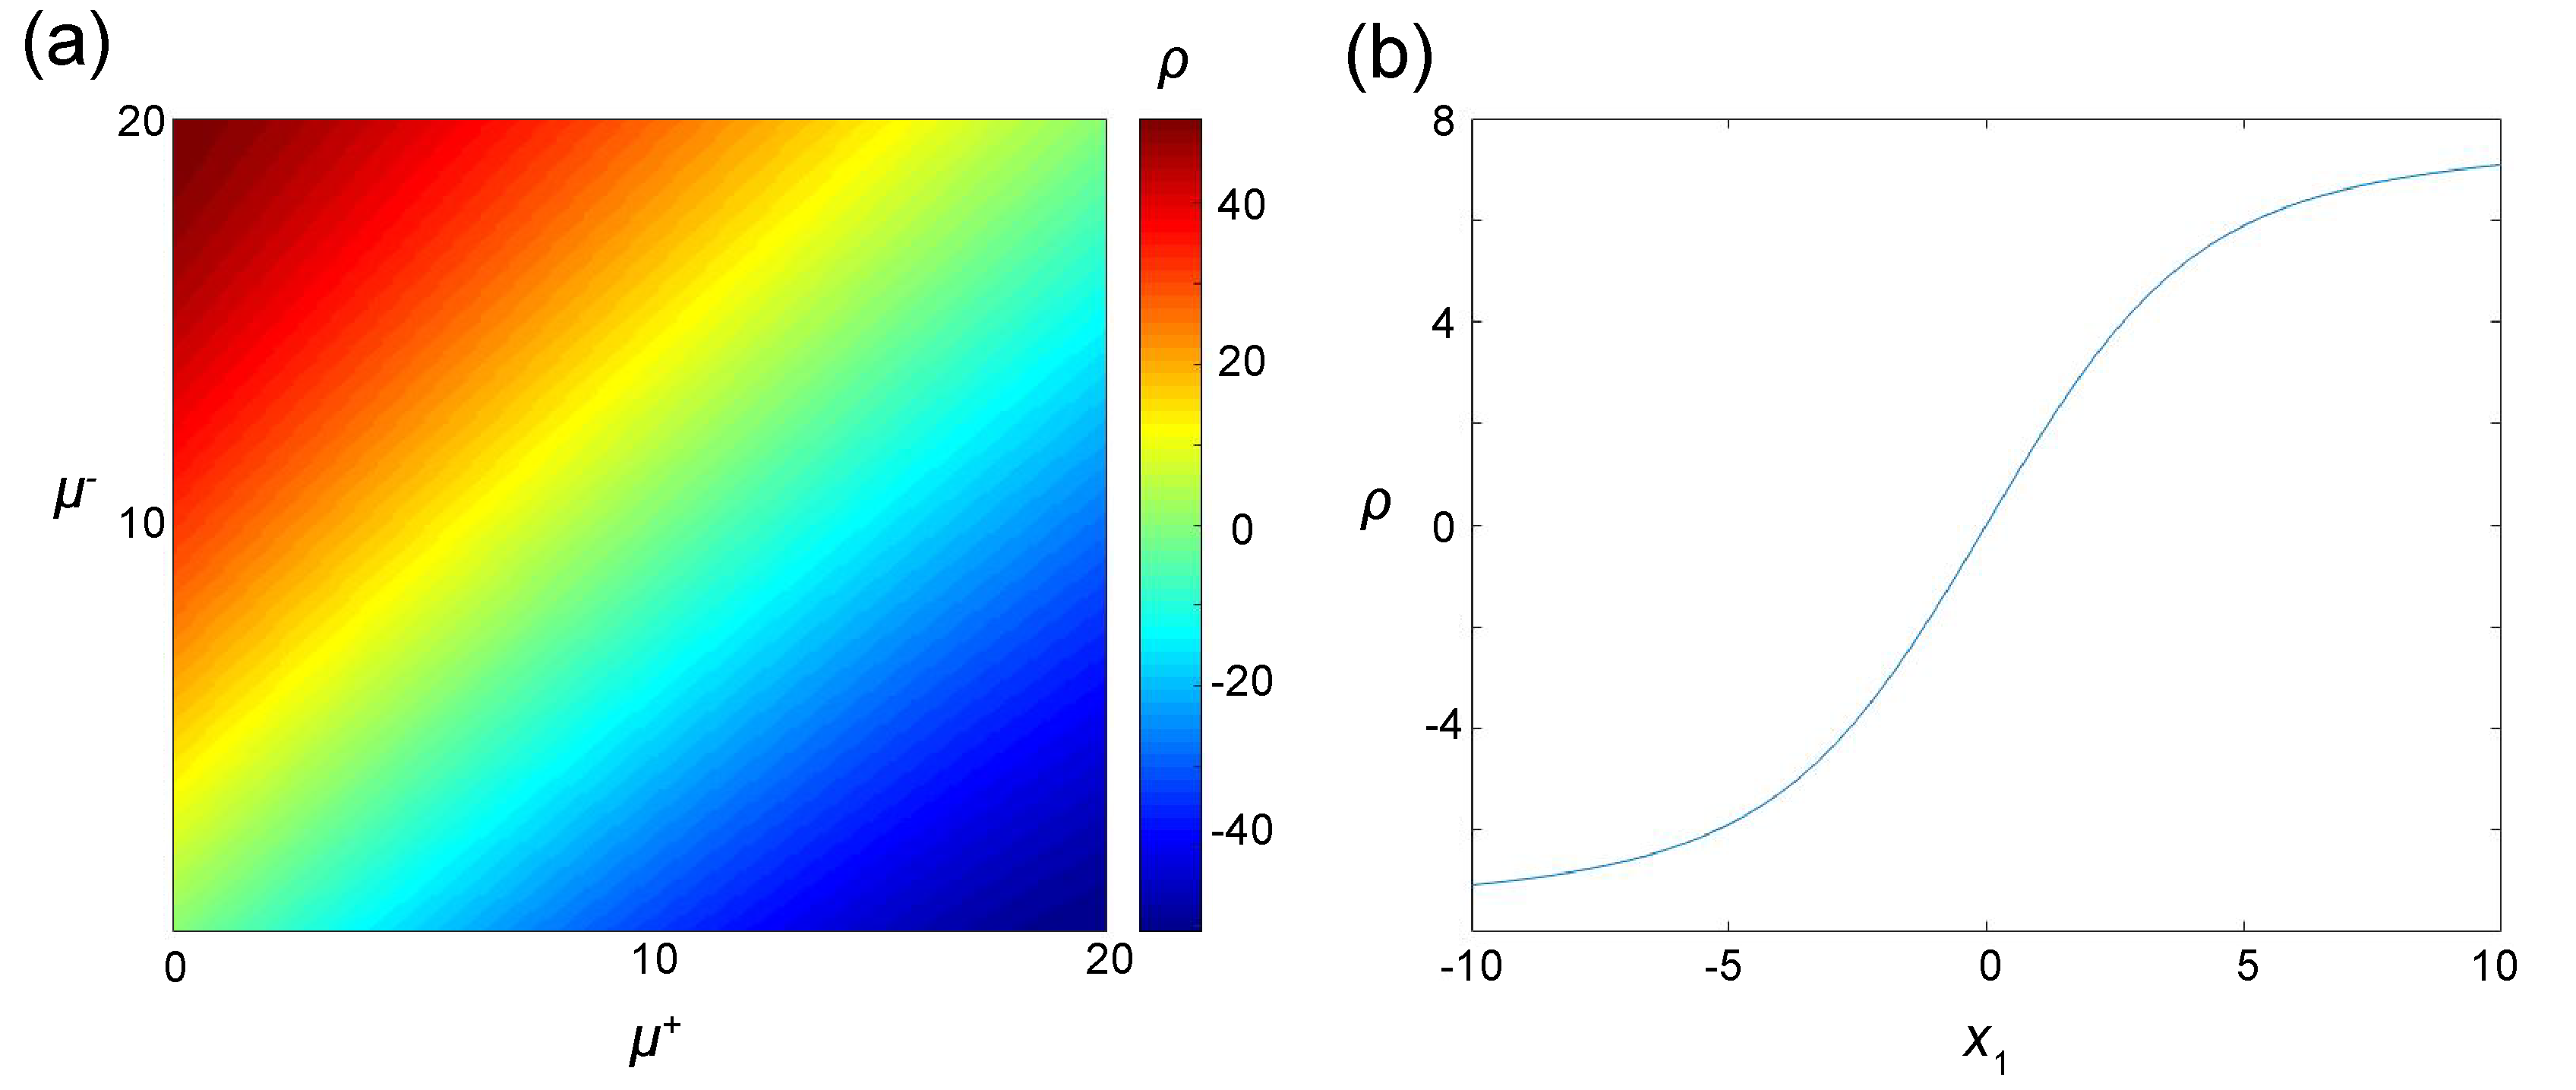
\includegraphics[scale=0.25]{chart/ratefunction.pdf}
	%\captionsetup{singlelinecheck = false, format= hang, justification=raggedright, font=footnotesize, labelsep=space}
	\caption{ST经验(净)环流的速率函数图像 (a) 三状态全连接马氏链,$\rho=I_Q(\cdots,\mu^+,\mu^-)-I_Q(\cdots,\mu^-,\mu^+)+(\log\frac{\gamma^+}{\gamma^-})(\mu^+-\mu^-)$的热力图,表明Gallavotti-Cohen 类型涨落定理对ST环流不成立。选择的参数是:$\mu^1=15, \mu^2=20, \mu^3=3, \mu^{12}=21, \mu^{23}=37, p_{11}=0.28, p_{12}=0.22, p_{13}=0.5, p_{21}=0.1,  p_{22} = 0.6, p_{23}=0.3, p_{31}=0.3, p_{32}=0.3, p_{33}=0.4$
    (b) 四状态全连接马氏链,$\rho=I_{\tilde{Q}}(\tilde{\mu}^{c_1},\tilde{\mu}^{c_2},\tilde{\mu}^{c_3})-  I_{\tilde{Q}}(-\tilde{\mu}^{c_1},\tilde{\mu}^{c_2},\tilde{\mu}^{c_3})+(\log\frac{\gamma^{c_1}}{\gamma^{c_1-}})\tilde{\mu}^{c_1}$的函数图像,表明Gallavotti-Cohen 类型涨落定理对ST净环流不成立。选择的参数是:$x_2 = 2, x_3 = 3, p_{11} = 0.1, p_{12} = 0.2, p_{13} = 0.3,p_{14} = 0.4,$ $p_{21} = 0.5, p_{22} = 0.15, p_{23} = 0.15, p_{24} = 0.2, p_{31} = 0.1, p_{32} = 0.4, p_{33} = 0.25, p_{34} = 0.25,
    p_{41} = 0.2, p_{42} = 0.2, p_{43} = 0.3, p_{44} = 0.3$}\label{figure:ratefunction}
\end{figure}
尽管ST经验环流无法满足各种涨落定理,ST经验净环流却是在很多情况下成立(参考 \cite{andrieux2007fluctuation})。对于单环系统,只需考虑环$C^+$的经验净环流$\tilde{Q}^+_n$。假设选定生成树为$T = 1 \rightarrow 2 \rightarrow \cdots N$。在周期边界条件下,由公式 \ref{conversion},可得$Q_n^+=J_n^- + J^{(N,1)}$和$Q_n^-=J_n^- + J^{(N,1)}$。这两个方程表明 $\tilde{Q}_n^+ = \tilde{J}_n^+$,因此 ST净环流的涨落定理自然可以由LE净环流的涨落定理得出。如果没有周期边界条件,Gallavotti-Cohen型涨落定理仍然成立,因为它反映了系统的长期行为,是否假设周期边界条件并不会影响大偏差速率函数,然而其他三种类型的涨落定理将不会成立。文献\cite{polettini2014transient} 表明,对于ST净环流,四种类型的涨落定理都成立。

上述结论可以扩展到一般马氏链。对于一元环和二元环,ST经验净环流为0,只需考虑有三状态或者更多状态的环。令$\{c_{l_1}, c_{l_2},\cdots, c_{l_s}\} \subset \mathcal{L}$表示基本集中所有三元环或多元环,那么环$c$及相应的反环$c^-$都只出现一次。事实上,文献\cite{andrieux2007fluctuation}已经证明了,ST净环流满足弱形式下的Gallavotti-Cohen型涨落定理:
\begin{equation} \label{Gallavotti}
    I_{\tilde{Q}}(x_1,x_2,\cdots,x_s)
    = I_{\tilde{Q}}(-x_1,-x_2,\cdots,-x_s)
    -\sum_{i=1}^s x_i\log\frac{\gamma^{c_{l_i}}}{\gamma^{c_{l_{i}-}}}.
\end{equation}
这说明ST经验净环流的联合分布满足对称关系。事实上,上述等式可以由LE净环流的涨落定理直接得出。对于任意三状态或者更多状态的环$c_l \in \mathcal{L}$,在周期边界条件下,由公式\ref{conversion},可得:
\begin{equation*}\label{circulation}
    \begin{split}
    \tilde{Q}^{c_l}_n =\sum_{c\ni l}J^c_n-\sum_{c\ni l-}J^c_n
    =\sum_{c\ni l}J^c_n-\sum_{c\ni l}J^{c-}_n = \tilde{J}^c_n.
    \end{split}
\end{equation*}
因此ST经验净环流可以分解为LE经验净环流的和。

%%%%%%%%%%%%%%%%%%%%%%%%%%%%%%%%%%%%%%%%%%%%%%%%%%%%%%%%%%%%%%%%%%%%%%%
% \subsubsection{经验LE环流的暂态涨落定理的证明}
% 在此,将给出无周期条件下,经验LE环流的暂态涨落定理的证明。
% 记 $k=(k^c)_{c\in\mathcal{C}}\in \mathbb{N}^{2N+2}$。在时间步 $n$,轨道中环 $c$ 形成 $k^c$ 次,因此有:
% \begin{equation*}
% 	n=\sum_{c\in\mathcal{C}}k^c|c|+|\eta|,
% \end{equation*}
% 其中 $\eta$ 表示剩下的导出链,且 $0\le |\eta|\le N-1$。假设系统从状态 1 出发,这并不降低命题的一般性。令 $[\eta]=t$,那么 $\eta=\eta_1$ 或者 $\eta_2$,其中 $\eta_1=[1,2,\cdots,t+1]$ 且 $\eta_2=[1,N,\cdots,N+1-t]$。同时, \eqref{joint} 可以被写为:
% \begin{equation}\label{joint2}
% 	\begin{split}
% 		\mathbb{P}\left(N^c_n=k^c,\;\forall c\in\mathcal{C}\right)
% 		=&\;\mathbb{P}\left(N^c_n=k^c,\;\forall c\in\mathcal{C},\tilde{\xi}_n=\eta_1\right)+\mathbb{P}\left(N^c_n=k^c,\;\forall c\in\mathcal{C},\tilde{\xi}_n=\eta_2\right)\\
% 		=&\;\left|G^{\eta_1}(k)\right|\left[\prod_{c\in\mathcal{C}}\left(\gamma^c\right)^{k^c}\right]\gamma^{\eta_1}+\left|G^{\eta_2}(k)\right|\left[\prod_{c\in\mathcal{C}}\left(\gamma^c\right)^{k^c}\right]\gamma^{\eta_2},
% 	\end{split}
% \end{equation}
% 其中 $\gamma^{\eta_1}=p_{12}\cdots p_{t,t+1}$ 且 $\gamma^{\eta_2}=p_{1N}\cdots p_{N+2-t,N+1-t}$。那么有
% \begin{align*}
% 	\mathbb{P}\left(N^+_n=k^+,N^-_n=k^-,\cdots\right)
% 	&= (\gamma^+)^{k^+}(\gamma^-)^{k^-}\prod_{c\neq C^+,C^-}\left(\gamma^c\right)^{k^c}\\
% 	&\qquad\left[|G^{\eta_1}(k^+,k^-,\cdots)|\gamma^{\eta_1}+|G^{\eta_2}(k^+,k^-,\cdots)|\gamma^{\eta_2}\right].
% \end{align*}
% 同理,如果交换上述方程中的 $k^+$ 和 $k^-$,可以得到:
% \begin{align*}
% 	\mathbb{P}\left(N^+_n=k^-,N^-_n=k^+,\cdots\right)
% 	&= (\gamma^+)^{k^-}(\gamma^-)^{k^+}\prod_{c\neq C^+,C^-}\left(\gamma^c\right)^{k^c}\\
% 	&\qquad\left[|G^{\eta_1}(k^-,k^+,\cdots)|\gamma^{\eta_1}+|G^{\eta_2}(k^-,k^+,\cdots)|\gamma^{\eta_2}\right].
% \end{align*}
% 根据 \eqref{EGetan} 式,可以得到下列的暂态涨落定理成立:
% \begin{equation*}
% 	\mathbb{P}\left(N^+_n=k^+,N^-_n=k^-,\cdots\right)=\mathbb{P}\left(N^+_n=k^-,N^-_n=k^+,\cdots\right)\left(\frac{\gamma^+}{\gamma^-}\right)^{k^+-k^-}.
% \end{equation*}
%%%%%%%%%%%%%%%%%%%%%%%%%%%%%%%%%%%%%%%%%%%%%%%%%%%%%%%%%%%%%%%%%%%%%%%%%%%%%%%%

% 由公式\ref{weak1},可得:

% 这表明周期边界条件下,ST净环流满足暂态涨落定理的弱形式。由于是否假设周期边界条件不会影响大偏差速率函数,则Gallavotti-Cohen类型涨落定理的弱形式 \cite{pedraza2008effects} 成立。


我们知道是否假设周期边界条件不会影响大偏差速率函数,因此Gallavotti-Cohen类型涨落定理的弱形式 \cite{pedraza2008effects} 成立。下面证明,在周期边界条件下,ST净环流满足暂态涨落定理的弱形式,即:
\begin{equation}\label{weak2}
    \begin{split}
    \frac{\Pnum\left(\tilde{Q}^{c_{l_1}}_n=x_1,\cdots, \tilde{Q}^{c_{l_s}}_n=x_{s}\right)}
    {\Pnum\left(\tilde{Q}^{c_{l_1}}_n=-x_1,\cdots, \tilde{Q}^{c_{l_s}}_n=-x_{s}\right)}
    =e^{n\sum_{i=1}^{s}x_i\log\frac{\gamma^{c_{l_i}}}{\gamma^{c_{l_i}-}}}.
    \end{split}
\end{equation}
%%%%%%%%%%%%%%%%%%%%%%%%%%%%%%%%%%%%%%%%%%%%%%%%%%%%%%%%%%%%%%%%%%%%%%%%%
% 接下来在周期边界条件下证明\ref{weak2}。
\begin{proof}
    由公式\ref{circulation},对任意三状态或者更多状态的环$c_l \in \mathcal{L}$,有:
\begin{equation*}
    \tilde{Q}_{n}^{c_{t}}=\sum_{i=1}^{r} \tilde{J}_{n}^{c_{i}}\left[1_{\left\{l \in c_{i}\right\}}-1_{\left\{l \in c_{i}-\right\}}\right]
\end{equation*}
其中$1_A$是指示函数,若A成立,则为1,否则为0。那么,可以得到:
\begin{equation*}
\begin{array}{l}
    \mathbb{P}\left(\tilde{Q}_{n}^{c_{l_{1}}}=x_{1}, \cdots, \tilde{Q}_{n}^{c_{l_{s}}}=x_{s}\right)\\
    =\mathbb{P}\left(\sum_{i=1}^{r} \tilde{J}_{n}^{c_{i}}\left[1_{\left\{l_{1} \in c_{i}\right\}}-1_{\left\{l_{1} \in c_{i}-\right\}}\right]=x_{1}, \cdots, \sum_{i=1}^{r} \tilde{J}_{n}^{c_{i}}\left[1_{\left\{l_{s} \in c_{i}\right\}}-1_{\left\{l_{s} \in c_{i}-\right\}}\right]=x_{s}\right)\\
    =\sum_{\sum_{i=1}^{r} y_{i}\left[1_{\left\{l_{m} \in c_{i}\right\}}-1_{\left\{l_{m} \in c_{i}-\right\}}\right]=x_{m}, 1 \leq m \leq s} \mathbb{P}\left(\tilde{J}_{n}^{c_{1}}=y_{1}, \cdots, \tilde{J}_{n}^{c_{r}}=y_{r}\right)\\
    =\sum_{\sum_{i=1}^{r} y_{i}\left[1_{\left\{l_{m} \in c_{i}\right\}}-1_{\left\{l_{m} \in c_{i}-\right\}}\right]=x_{m}, 1 \leq m \leq s} \mathbb{P}\left(\tilde{J}_{n}^{c_{1}}=-y_{1}, \cdots, \tilde{J}_{n}^{c_{r}}=-y_{r}\right) e^{n \sum_{i=1}^{r} y_{i} \log \frac{\gamma^{c_{i}}}{\gamma^{c_{i}-}}}\\
    =\sum_{\sum_{i=1}^{r} y_{i}\left[1_{\left\{l_{m} \in c_{i}\right\}}-1_{\left\{l_{m} \in c_{i}-\right\}}\right]=x_{m}, 1 \leq m \leq s} \mathbb{P}\left(\tilde{J}_{n}^{c_{1}}=-y_{1}, \cdots, \tilde{J}_{n}^{c_{r}}=-y_{r}\right) e^{n \sum_{i=1}^{s} x_{i} \log \frac{\gamma^{c_{l_i}}}{\gamma^{c_{l_i}-}}}\\
    =\sum_{\sum_{i=1}^{r} y_{i}\left[1_{\left\{l_{m} \in c_{i}\right\}}-1_{\left\{l_{m} \in c_{i}-\right\}}\right]=-x_{m}, 1 \leq m \leq s} \mathbb{P}\left(\tilde{J}_{n}^{c_{1}}=y_{1}, \cdots, \tilde{J}_{n}^{c_{r}}=y_{r}\right) e^{n \sum_{i=1}^{s} x_{i} \log \frac{\gamma^{c_{l_i}}}{\gamma^{c_{l_i}-}}}\\
    =\mathbb{P}\left(\sum_{i=1}^{r} \tilde{J}_{n}^{c_{i}}\left[1_{\left\{l_{1} \in c_{i}\right\}}-1_{\left\{l_{1} \in c_{i}-\right\}}\right]=-x_{1}, \cdots, \sum_{i=1}^{r} \tilde{J}_{n}^{c_{i}}\left[1_{\left\{l_{s} \in c_{i}\right\}}-1_{\left\{l_{s} \in c_{i}-\right\}}\right]=-x_{s}\right) e^{n \sum_{i=1}^{s} x_{i} \frac{\gamma^{c_{l_i}}}{\gamma^{c_{l_i}-}}}\\
    =\mathbb{P}\left(\tilde{Q}_{n}^{c_{l_{1}}}=x_{1}, \cdots, \tilde{Q}_{n}^{c_{l_{s}}}=x_{s}\right) e^{n \sum_{i=1}^{s} x_{i} \log \frac{\gamma^{c_{l_i}}}{\gamma^{c_{l_i}-}}},
\end{array}
\end{equation*}
在约束 $\sum_{i=1}^{r} y_{i}\left[1_{\left\{l_{m} \in c_{i}\right\}}-1_{\left\{l_{m} \in c_{i}-\right\}}\right]=x_{m}, 1 \leq m \leq s$下,我们使用了下面等式推出上面公式:
\begin{equation} \label{constraint}
    \sum_{i=1}^{r} y_{i} \log \frac{\gamma^{c_{i}}}{\gamma^{c_{i}-}}=\sum_{j=1}^{s} x_{j} \log \frac{\gamma^{c_{l_{j}}}}{\gamma^{c_{l_{j}}-}}
\end{equation}
这个等式是非平凡的,我们接下来下面会证明它。对于任意环$c$,令$L^c$为E上的函数:
\begin{equation*}
    L^{c}(i, j)= \begin{cases}1, & \text { if }\langle i, j\rangle \in c \\ 0, & \text { otherwise }\end{cases}
\end{equation*}
通过$H^c$的定义,我们可以证明 \cite{kalpazidou2007cycle}:
\begin{equation*}
    L^c = \sum_{l \notin T} L^c(l) H^{c_l}
\end{equation*}
令E上的函数$w$定义为:
\begin{equation*}
    w(i, j) = \log \frac{p_{ij}}{p_{ji}}
\end{equation*}
对任意环 $c=(i_1, i_2, \cdots, i_t)$,有:
\begin{equation*}
    \log \frac{\gamma^{c}}{\gamma^{c-}} = \sum^t_{k=1} \log \frac{p_{i_k, i_{k+1}}}{p_{i_{k+1}, i_k}} = \langle w, L^c \rangle,
\end{equation*}
其中$i_{t+1} = i_1$,且 $\langle w, L^c \rangle = \sum_{\langle i, j \rangle \in E} w(i,j) L^c(i,j)$表示内积。此外,对于任意环$c_l \in \mathcal{L}$,很难证明:
\begin{equation*}
    \log \frac{\gamma^{c_l}}{\gamma^{c_l -}} = \langle w, H^{c_l} \rangle
\end{equation*}
注意到对任意一元环和二元环,有$\log (\gamma^c / \gamma^{c-})$。那么对任意环$c$,有:
\begin{equation*}
    \sum_{j=1}^{s}\left[L^{c}\left(l_{j}\right)-L^{c-}\left(l_{j}\right)\right] \log \frac{\gamma^{c_{l_{j}}}}{\gamma^{c_{j}-}}=\sum_{l \notin T} L^{c}(l) \log \frac{\gamma^{c_{l}}}{\gamma^{c_{l}-}}
\end{equation*}
因此最终可得:
\begin{equation*}
    \begin{aligned}
    \sum_{j=1}^{s} x_{j} \log \frac{\gamma^{c_{i}}}{\gamma^{c_{i}-}} &=\sum_{j=1}^{s} \sum_{i=1}^{r} y_{i}\left[L^{c_{i}}\left(l_{j}\right)-L^{c_{i}-}\left(l_{j}\right)\right] \log \frac{\gamma^{c_{i}}}{\gamma^{c_{i}-}} \\
    &=\sum_{i=1}^{r} y_{i} \sum_{j=1}^{s}\left[L^{c_{i}}\left(l_{j}\right)-L^{c_{i}-}\left(l_{j}\right)\right] \log \frac{\gamma^{c_{i}}}{\gamma^{c_{i}-}} \\
    &=\sum_{i=1}^{r} y_{i} \sum_{l \notin T} L^{c_{i}}(l)\left\langle w, H^{c_{l}}\right\rangle \\
    &=\sum_{i=1}^{r} y_{i}\left\langle w, \sum_{l \notin T} L^{c_{i}}(l) H^{c_{l}}\right\rangle \\
    &=\sum_{i=1}^{r} y_{i}\left\langle w, L^{c_{i}}\right\rangle=\sum_{i=1}^{r} y_{i} \log \frac{\gamma^{c_{i}}}{\gamma^{c_{i}-}}
    \end{aligned}
\end{equation*}
\ref{constraint}得证,同时弱形式暂态涨落定理的证明也完成了。

\end{proof}


%%%%%%%%%%%%%%%%%%%%%%%%%%%%%%%%%%%%%%%%%%%%%%%%%%%%%%%%%%%%%%%%%%%%%%%%%

对比LE经验净环流,我们能够发现ST经验净环流不满足强形式下的 Gallavotti-Cohen 类型涨落定理,可以参考文献 \cite{mehl2012role,polettini2017effective,uhl2018fluctuations,kahlen2018hidden}。我们考虑图 \ref{figure:transitiongraph}(b) 中的具有全连接的四状态马氏链,可以举出反例。对于一个环,基本集中只有它的反环,一元环和二元环,所以选定生成树为 $T=1\to2\to3\to4$,只需考虑三个环$c_1=(1,2,3)$,$c_2=(2,3,4)$和$c_3=(1,2,3,4)$的ST净环流。回顾ST经验净环流的速率函数$(\tilde{Q}_n^{c_1}, \tilde{Q}_n^{c_2}, \tilde{Q}_n^{c_3})$为:
\begin{equation}
	I_{\tilde{Q}}(x)=\inf_{\{\mu\in\mathcal{M}:\mu^{c_i}-\mu^{c_i-}= x_i,\forall 1\le i\le 3\}}I_Q(\mu).
\end{equation}

在选定适当参数下,图\ref{figure:ratefunction}(b)展现了,$I_{\tilde{Q}}(x_1, x_2, x_3)$ 和 $ I_{\tilde{Q}}(-x_1, x_2, x_3) -\left(\log \gamma^{c_1} / \gamma^{c_1-}\right)\tilde{\mu}^{c_1}$之间的差异。易知,两者差值非零,因此有:
\begin{equation}
    I_{\tilde{Q}}(x_1, x_2, x_3) \neq I_{\tilde{Q}}(-x_1, x_2, x_3) -\left(\log\frac{\gamma^{c_1}}{\gamma^{c_1-}}\right)\tilde{\mu}^{c_1},
\end{equation}
因此ST经验净环流不满足 Gallavotti-Cohen 类型涨落定理的强形式。
}

% !Mode:: "TeX:UTF-8" 

\BiAppendixChapter{致\quad 谢}{Acknowledgements}

% 三年的硕士生涯即将画上句号。在这里,我要向这期间曾经帮助过我的人,表达最诚挚的谢意。

% 首先,我要感谢我的导师张智民老师,还有在学术研究中指导过我的 李会元老师,许志钦老师,孙继广老师,蔡伟老师,贾晨老师(排名不分先后)。这些老师们无论是在学术方面还是生活方面,都给了我很多的指导和关心。而我也在这些老师身上学到的也不只是学术知识,更多的是严谨求实的态度和为人处世的道理。他们的言传身教使我终生受益。

% 同时,我也要感谢这三年来与我一起学习的各位同窗。在我面对困难灰心丧气的时候,他们总是给陪在我身边,给了我许许多多的鼓励。感谢他们陪我度过了一段永生难忘的岁月。

% 此外,我还要感谢我的家人和我的父母,他们是我在科研道路上的坚实后盾。感谢他们在硕士期间给了我充分的自由。我衷心希望自己能真正地成为家人眼中的骄傲。

% 最后,我要感谢我未来的女朋友。感谢她在我三年的硕士生涯中从来没有和我恋爱,使我可以专心地从事学术研究工作。

% 三年前,不知什么原因让我执着地来到了这里,可能是科研兴趣,可能是当时家庭变故,也可能只是想为慌乱的心灵找一个可以安静地方。这么说,并不是过分夸张,我本科的朋友不理解我为什么来到此处做这个方向;研究生的同学和老师对我的评价是,你在这条路好像可以走下去,但并不是很适合;找工作面试我的HR也问我,你为什么去那个地方读研。好像每次解释这件事的时候,我说的都不是很一致
% 三年即将结束,三年时间很漫长,甚至有些不承认这只是三年,他不是很精彩,却依然丰富。


% 不敢谈英雄主义,三年让我认清了些生活的真相,也不减对生活的热爱。   % 致谢


\defaultfontsmall
\bibliographystyle{GBT7714-2005NLang}
\addcontentsline{toc}{chapter}{参考文献}      % 参考文献加入到中文目录
\addcontentsline{toe}{chapter}{References}    % 参考文献加入到英文目录
\addtolength{\bibsep}{-0.8em}
%\nocite{*}  %若将此命令屏蔽掉,则未引用的文献不会出现在文后的参考文献列表中。
\bibliography{reference}

% !Mode:: "TeX:UTF-8"

\BiAppChapter{攻读\cxuewei 学位期间发表的论文及其他成果}{}
\setlength{\parindent}{0em}
\textbf{(一)发表的学术论文}
\begin{publist}
\item Yuhao Jiang, Bingjie Wu, Chen Jia. Large deviations and fluctuation theorems for cycle currents defined in the loop-erased and spanning tree manners: a comparative study. (Submitted)
\end{publist}

\textbf{(二)参加学术活动情况}
\begin{publist}
\item 2019年度北京大学“应用数学专题讲习班”
\item 2020年“基于机器学习的PDE数值计算与应用”暑期短课程
\item 2020年江苏省研究生“科学计算与大数据分析”暑期学校
\item 2020年度北京大学“应用数学专题讲习班”
\item 2021年南开大学散射与反散射暑期短期课程
\item 机器学习和大数据在复杂性科学中的应用暑期培训班
\end{publist}
\vfill
\hangafter=1\hangindent=2em\noindent

\setlength{\parindent}{2em}
    % 所发文章

\ifxueweidoctor
% !Mode:: "TeX:UTF-8"


\BiAppChapter{个人简历}{Resume}

XXXX~年~XX~月~XX~日出生于~XXXX。

XXXX~年~XX~月考入~XX~大学~XX~院(系)XX~专业,XXXX~年~XX~月本科毕业并获得~XX~学学士学位。

XXXX~年~XX~月------XXXX~年~XX~月在~XX~大学~XX~院(系)XX~学科学习并获得~XX~学硕士学位。

XXXX~年~XX~月------XXXX~年~XX~月在~XX~大学~XX~院(系)XX~学科学习并获得~XX~学博士学位。

获奖情况:如获三好学生、优秀团干部、X~奖学金等(不含科研学术获奖)。

工作经历:

\vspace{3em}\noindent
\textbf{( 除全日制硕士生以外,其余学生均应增列此项。个人简历一般应包含教育经历和工作经历。)}
          % 博士学位论文有个人简介
\fi

\clearpage

\end{document}
